\documentclass[12pt]{article}
\usepackage[english]{babel}
\usepackage[utf8x]{inputenc}
\usepackage{amsmath}
\usepackage{amsfonts}
\usepackage{graphicx}
\usepackage{float}
\usepackage{subcaption}
\usepackage[colorinlistoftodos]{todonotes}
\usepackage{algorithm}
\usepackage{algpseudocode}
\usepackage{amssymb}
\usepackage{url}
 
\begin{document}
\begin{titlepage}
\newcommand{\HRule}{\rule{\linewidth}{0.5mm}}
\center 
\textsc{\LARGE University at Buffalo, The State University of new York}\\[1.5cm] 
\textsc{\Large CAL @ UB}\\[0.5cm] 
\textsc{\large Master of Science Project Report}\\[0.5cm] 
\HRule \\[0.3cm]
{ \LARGE \bfseries Path Planning and Motion Control for Autonomous Mobile Robots}\\[0.3cm] 
\HRule \\[1.2 cm]
\begin{minipage}{0.4\textwidth}
\begin{flushleft} \large
\emph{Author:}\\
Swapneel Bhavesh \textsc{Mehta} % Your name
\end{flushleft}
\end{minipage}
~
\begin{minipage}{0.4\textwidth}
\begin{flushright} \large
\emph{Supervisor:} \\
Dr. Minghui \textsc{Zheng}
\end{flushright}
\end{minipage}\\[2cm]
{\large \today}\\[2 cm] 
\begin{figure}[ht]
\begin{subfigure}{0.5\textwidth}
    
\includegraphics[width=0.6\linewidth, height=2.6cm]{UB_LOGO.png} 
\end{subfigure}
\begin{subfigure}{0.5\textwidth}

\includegraphics[width=0.6\linewidth, height=2.2cm]{CAL@UB.jpeg}
\end{subfigure}
\end{figure}

\vfill
\end{titlepage}

\begin{titlepage}
\section*{\centering\sc{acknowledgement}}
I would first like to thank my project advisor Assistant Professor, Dr Minghui Zheng of the Department of Mechanical and Aerospace Engineering at 'University at Buffalo'. The door to Prof. Zheng's office was always open whenever I ran into a trouble spot or had a question about my research or writing. She provided LAB equipment, instruments and devices that were required for research. She also consistently allowed this paper to be my own work, but steered me in the right direction whenever she thought I needed it.\par \noindent \\
I would also like to thank my CAL lab mates who always motivated the research by pointing out important notes during lab meetings. It was truly inspiring and great discussing ideas and working with them all the time. \par \noindent \\
I would also like to acknowledge Assistant Professor Dr Francis Lagor of the Department of Mechanical and Aerospace at 'University at Buffalo' for being an important part of the committee for project defense, and I am gratefully indebted to him for his very valuable comments on this work.\par \noindent \\
Finally, I must express my very profound gratitude to my parents, and my little sister for providing me with unfailing support and continuous encouragement throughout my years of study and through the process of researching and completing this project. This accomplishment would not have been possible without them. Thank you!
\par
\par \noindent \\
Swapneel Bhavesh Mehta
\end{titlepage}
\newpage

\begin{abstract}
This is a final report submitted to the academic advisor Dr. Minghui Zheng, in accordance to my research work done in CAL (control and Autonomous Laboratory) at University at Buffalo, during the year 2018. It includes Introduction to current problems in Robotics research field in beginning, following to which is some detailed overview of some of the Motion Planning Algorithms, implementation of developed/modified algorithms making use of V-Rep Robot simulator. Having a proper understanding of Motion Planning, dynamic analysis with mathematical formulation is presented later on, following which some control techniques and simulation results using MATLAB is also presented. Thus, everything that a Robot needs to become Autonomous including Planning, System Integration, Implementation and Controlling is developed and combined to simulate a robot and that concludes this whole report.  
\end{abstract}
\newpage

\section{Introduction}
Robotics, a field of applied science integrating Mechanical Engineering, Electrical Engineering and Computer Science, solves the problems including design, construction, operation and various applications of robots. Various systems when configured and integrated in a single system, makes a robot perform the desired tasks that prove to be helpful for human kind in many different ways. There are many different types of robot models being designed and developed day by day in modern robotics field. Fixed base, robot manipulators used in industrial applications, mobile base, mobile robots including autonomous vehicles, wheeled robots, legged robots, humanoid robots, are used in a lot of applications.
\par \noindent 
Latest research has developed a mobile manipulator robot, used in military, marine, used as Bomb Disposal robot. These robots are a game changer in today's world. These robots are capable of performing tasks that could be dangerous to humans, such as disposing a bomb, entering into a building with a hostage situation, or dealing with any poisonous or explosive devices. The design of this robot looks something like a wheeled or a cannon like base with a manipulator arm mounted  on top which performs the tasks desired. 
 \subsection{Planning in robotics}
Motion Planning is a very important term in Robotics with a general definition given as automation of mechanical systems by integrating sensing, actuation and computational capabilities. "Autonomous systems" is a term which closely relates to this definition, any system that design or creates a plan itself and follows that plan to execute the desired operation precisely. Algorithms are used to command the robots to make the plan based on instructions provided. Robot motion planning generally ignores the dynamics, limitations and constraints on mechanical or the dynamic model. So, in short, it just plans different types of movements such as translation and rotation along the available path.  \par \noindent
Trajectory planning is a different problem that takes the solution from motion planning problem, and determines how to move along planned path considering constraints and limitations of robot. Trajectory planning takes time as a parameter, it solves for velocity and acceleration at each instant of time and not just plans the path from initial and goal positions. It could be either discrete or continuous based on ease and credibility of the situation to be handled by robot. Any dynamic and motion constraints are taken care of during trajectory planning problem. 
\par \noindent
Collision detection and avoiding any obstacle is one of the steps of planning problem. It is obvious that a mobile robot when moving around in a configuration space will come across some object at some point and optimal path may be colliding with that obstacle. This is not safe, so it is more important to avoid those collision than to design shortest path for the robot. Algorithms used for planning must implement a limitation on the robot to not modify the path if it is intersecting with any coordinates that represents the position of any of the obstacles visible on map. 
\par \noindent
So, overall problem of planning in robotics is finding a minimum cost path or trajectory which leads the robot from an initial state to desired goal state in minimum time along with avoiding any obstacles that might happen to be in robot's way. Dynamics of the model is required while trajectory planning and controlling. Control theory with feedback technique is used generally to make sure the robot is following the planned path and performing desired operation. 
\subsection{Robot's environment}
Different robotic problems have different environment in which the robot has to work. First of all, Configuration space or C-space is the space in which robot can move around and perform any tasks and it is bounded by the robot's limitations.  Sometimes, the map of C-space is already available before hand and the space is rigid, which means there is no any moving object and everything is fixed and known. This is generally indoor or within an enclosed field. Then there is a dynamic Environment which includes humans, vehicles, other living beings and even other robots. This problem requires a special attention. Rarely, but possible case is that the Environment is totally unknown before putting the robot in C-space. Vision sensor and artificial intelligence and use of machine learning algorithms is required along with planning.
\par \noindent
Among mobile vehicle type robots, two types of planning algorithms are popular, grid based planning and sampling based planning. In grid based planning, the C-space is divided into partitioned layers, which forms nodes and edges to obtain path for the robot. While, in sampling based planning, nodes are designed by algorithm and then selected nodes are used to plan the path optimizing the objective function.
\subsection{Dynamics and control}
Dynamic model of a robot is derived by considering forces acting on and by the system and motion of the robot in specific direction. The dynamic equations of robot model helps solving for the control problem in system and gives a proper understanding of the robot system. These equations are also known as equations of motion. A controller is designed by performing some analytic or mathematical derivations. Using the solution of motion planning as input here, states are updated with time steps. Using feedback error dynamics parameter, control is designed to minimize that error and stabilize the system. The error is calculated using the difference in desired parameters and actual values of parameters.
\par \noindent
Inverse dynamics and control procedure prove to be inefficient when dealing with uncertain parameters. Which means, the forces acted upon the system are unknown and that replace few variables in equations of motion with unknown quantity which brings the need to use advanced control techniques. Robust and Adaptive controls are some of the most advanced control in motion control problem. Robust control method is used when uncertainties found in parameters are within some fixed bounded set. While Adaptive control technique is more useful as it adapts the control law as per variations in measurements of parameters. Performance of the controller vary based on the changes in uncertainties. Generally, it uses parameter estimation technique to estimate the measurement before adapting to the updated control law.
\section{Planning algorithms (Motion planners)}
As mentioned before, there are some of the popular algorithms in robotics which are very useful in path planning and motion planning for mobile robots. 
\subsection{Grid based A-star search algorithm}
A-star is a computer algorithm widely used in finding an optimal path in between multiple nodes. The C-space for a robot could be represented using a graph consisting of nodes and edges representing paths divided in small instances. The graph space can be divided in free space and obstacle space, based on location of any obstacles in the map. Each edge has a different cost-to-go assigned based on different parameters related to robot. Starting from the initial node position, it finds next node to be travel to by identifying minimum cost edge. In such a way, by finding parent nodes, to reach to goal position with minimum costs this algorithm converges and obtains solution.   
\par \noindent
Lists are formed in this algorithm named as open list and closed list. Initially, All the nodes are unexplored which means each nodes are in open list and and closed list is empty and list fills up as we explore the nodes one by one. A sample algorithm is shown later for A-star graph search.
\begin{algorithm}[ht]
\caption{A-star search algorithm}
\begin{algorithmic}[1]
\State{initialization - All nodes in open list, O and closed list, C=empty}
\While{open list, O $\ne$ empty}
\State Chose a node  $N_{best} \mid  f(N_{best}) \leq f(N)$ \Comment{N=all neighbours}
\State{$O(N_{best}=\emptyset$)} \Comment{$N_{best}$ is removed from Open list}
\State{$C=C+N_{best}$} \Comment{$N_{best}$ is added to closed list}
\While{$N_{best} \ne Goal node$}
\For{$X \notin C $}
\State{Expand for X  in neighbour set  of $N_{best}$ }
\If{$X \notin O$}
\State{$O=O+X$}
\Else
\State{Update the parent of x as $N_{best}$ }
\State{And update the cost to reach to that node}
\EndIf
\EndFor
\EndWhile
\EndWhile
\end{algorithmic}
\end{algorithm}

\subsection{Sampling based motion planners}
Similar to grid based search algorithm, this sampling based planner works and delivers even better results. For systems having more number of degrees of freedom, grid based search is unsuitable and that is when sampling based search Planners are useful. These planners are also more useful in implementing collision avoidance during path finding. Configuration space of mobile robot is sampled uniformly to obtain more detailed information about the map and obstacles data. Solution obtained using these type of planners is more accurate and nearest to optimum. Additionally, obstacle avoidance technique could be easily implemented in it. There are major two types of sampling based search algorithms, namely, Probabilistic Road Map (PRM) and Randomly-explored Random Tree (RRT).
\subsubsection{Probabilistic road map algorithm (PRM) planner}
Initially, the algorithm builds a road map using only $C_{free}$ space, which is the space free of obstacles. After building this road map, local planners for instance A* search algorithm is used to find paths locally within samples. So, first of all, single query planner works on building obstacle free map to search using multiple queries path up till the final goal node. After map is built, then closest node is connected to the starting node adding it to the graph. Then the graph is searched for an optimal path to connect those nodes using a local planner. Thus, the solution is efficient and obtained quickly.  
\subsubsection{Random-exploring random tree (RRT) algorithm}
Major difference between PRM and RRT algorithms is that PRM makes use of road map graph with multiple query planning while RRT simply searches in tree like flow and single query motion planning. RRT algorithm has a good capacity of collision free path finding using kinematics and even dynamic planning. so, this type is more popular when forces and torques are to be considered while planning. The algorithm has a tree like structure which starts from a single starting node and searches within branches of neighbours for a optimal plan. Important point is formation of nodes which is done randomly all along the map. As sampling is done randomly, it takes less time to initialize the search and hence it is faster than PRM. RRT algorithm in its most generalized form is shown here.

\begin{algorithm}[ht]
\caption{RRT search algorithm}
\begin{algorithmic}[1]
\State{initialization - Begin searching using a tree, $T$ with node $x_{start}$}
\While{$T \leq $ Max tree size}
\State Chose random sample $x_{sample}  \longleftarrow  X$
\Comment{X is set of all samples}
\State{Find a node nearest to $x{sample}$ node, $x_{nearest}$ in $T$} \Comment{Branching}
\If{$x_{nearest}$ is not too far from $x_{sample}$}
\State{Use a local planner, A* to find motion from $x_{nearest}$ to $x_{sample}$} 
\Else{find motion from $x_{new}$ to $x_{nearest}$, in the direction same as $x_{sample}$}
\EndIf
\If{Motion found is obstacle-free}
\State{Add $x_{new}$ to the tree, $T$ with the path/edge found}
\If{$x_{new} \in X_{goal}$}\;
\Comment{$X_{goal}$ is set within final state}
\\
\Return{Path found successfully, and display the motion}
\EndIf
\EndIf
\EndWhile
\\
\Return{Failed to find a path}
\end{algorithmic}
\end{algorithm}
In this way, RRT algorithm keeps branching either up to the maximum number of iterations, maximum size of the tree is reached or goal node is caught in the tree. Every time direction of path remains the same and consistent even if the distance is too far, so using shorter random samples, it becomes very convenient and easy for local planner to plan a optimal path within those intervals. It depends on the program, how a sample the map, identify nearest nodes out of the pool of nodes and what planner to be used to reach up to sample node from the nearest node. The efficiency of algorithm sometimes also depends on given definition of how much far the nearest should be from the sample node. 
\par \noindent
There are different variants of RRT algorithms developed, one is bidirectional RRT, as the name suggests this planner searches for a path from both directions. The two directions of search are from starting state and other from goal state, both searches trying to find sample nodes in other direction. So, both of these planners meet at a certain point making a total optimal path. As the other search starts from goal node, exact goal will be reached rather than set of points within a range of goal position as in regular RRT. 
\par \noindent
Another type is RRT star algorithm, this is same as regular planner except the step where it returns success as soon as $X_{goal}$ set has reached and converges to that solution. In this modification, algorithm continues to search for optimal path using more number of nodes without converging to set of points. The only convergence condition is maximum size of tree or maximum number of nodes on map. In this planner, after obtaining $x_{new}$, it will search for neighbours in a range which could be reached with cost lower than that. In this manner, Even though, RRT* takes longer time to converge and obtain the solution, lowest cost edge will be connected to form the path and final motion will be more optimal compared to previous one. 

\section{Simulation results}
\subsection{Implementing A-star search algorithm}
Using the A-star search algorithm, taking into consideration, a bounded map with circular obstacles, nodes and edges data are provided. Using MATLAB program, A-star search method is implemented to find a shortest path without any collision. From the initial point of KILO-BOT it finds lowest cost path possible and it reaches to desired goal position.\;
\begin{figure}[H]
\centering
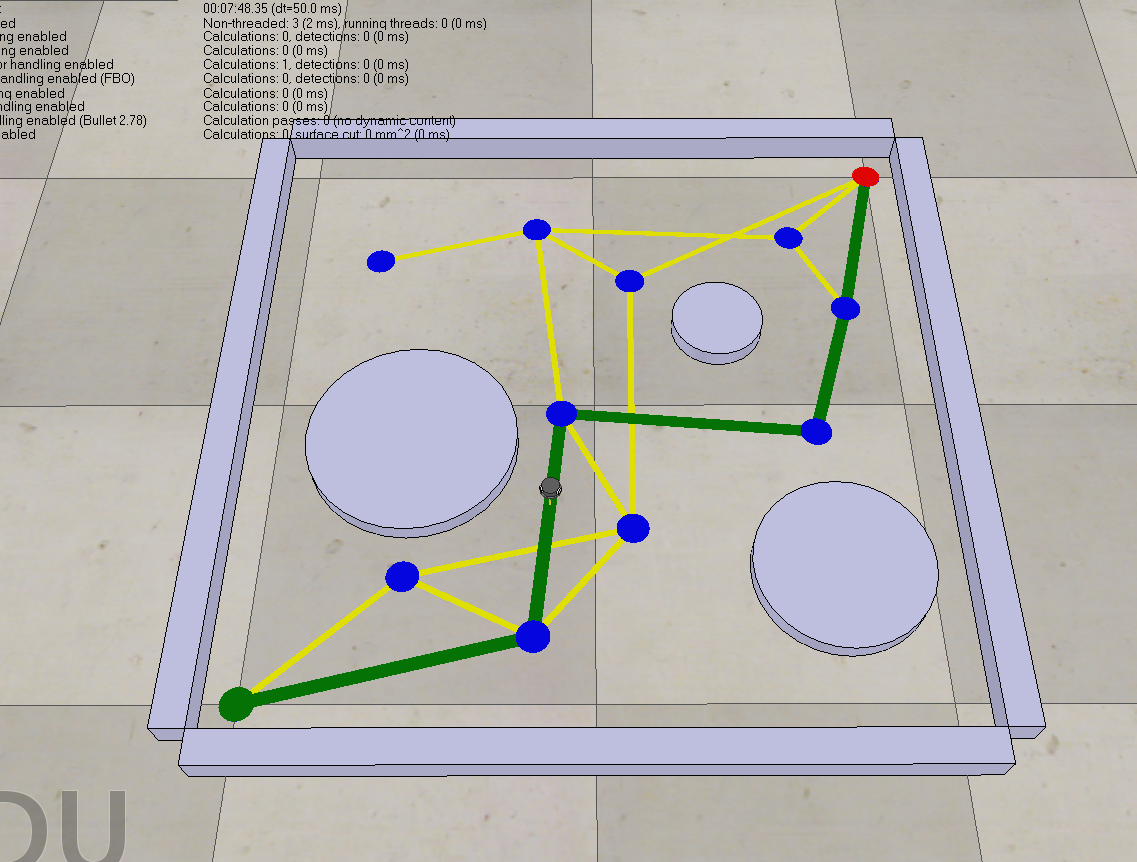
\includegraphics[scale=0.4]{VREP_Screenshot.png}
\captionsetup{labelformat=empty}
\caption{Screen shot of V-Rep simulation of A-star planner using Kilo-Bot}
\end{figure}
Input to program consists of obstacles, nodes, and edges data. Initially, all the nodes are put in open list and closed list is empty. Starting from first node and calculating to go costs from each parent nodes and reaching to goal node. The program gives the path data with nodes list that turns out to be minimum cost bearing solution. The output is produced as a Comma Separated Values (CSV) file which is sent to a robot simulator software, V-Rep to visualize the simulation on Kilo-Bot.    
\subsection{RRT algorithm implemented}
Sai Vemprala has created RRT Algorithm and uploaded in Mathworks website, using some of their work RRT search algorithm is developed and used for planning an optimal path with obstacle avoidance technique for mobile robots. The MATLAB program written for RRT implementation takes starting point, goal point, map coordinates and obstacles data as input. A function called 'move' explore the nodes in neighbourhood of random sample node to find and reach up to nearest node. Another function is used to avoid  any obstacles in the map, it directly eliminates any possibilities of exploring into the position where any obstacle intersects with the path. Nearest node from the sample node is found using distance function which calculates the distance between the nodes. Comparing calculated distances and selecting minimum distance node to move further the search and branching the tree, if obstacle is not interrupting the motion. 

\begin{figure}[H]
\begin{subfigure}{0.5\textwidth}
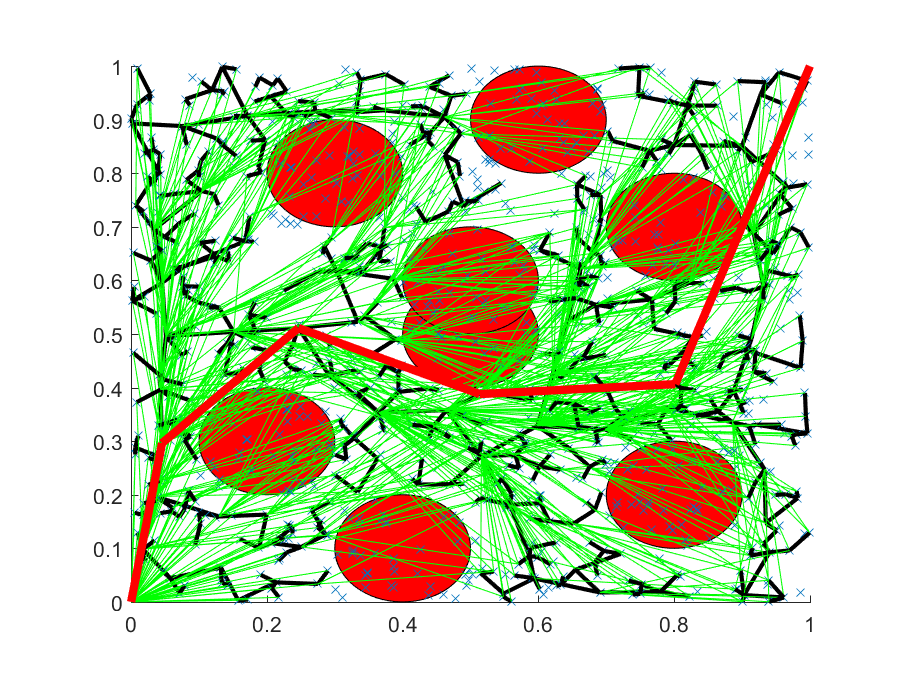
\includegraphics[width=0.7\linewidth, height=3.5cm]{matlab_plot.eps}
\captionsetup{labelformat=empty}
\caption{RRT MATLAB Plot}
\end{subfigure}
\begin{subfigure}{0.5\textwidth}
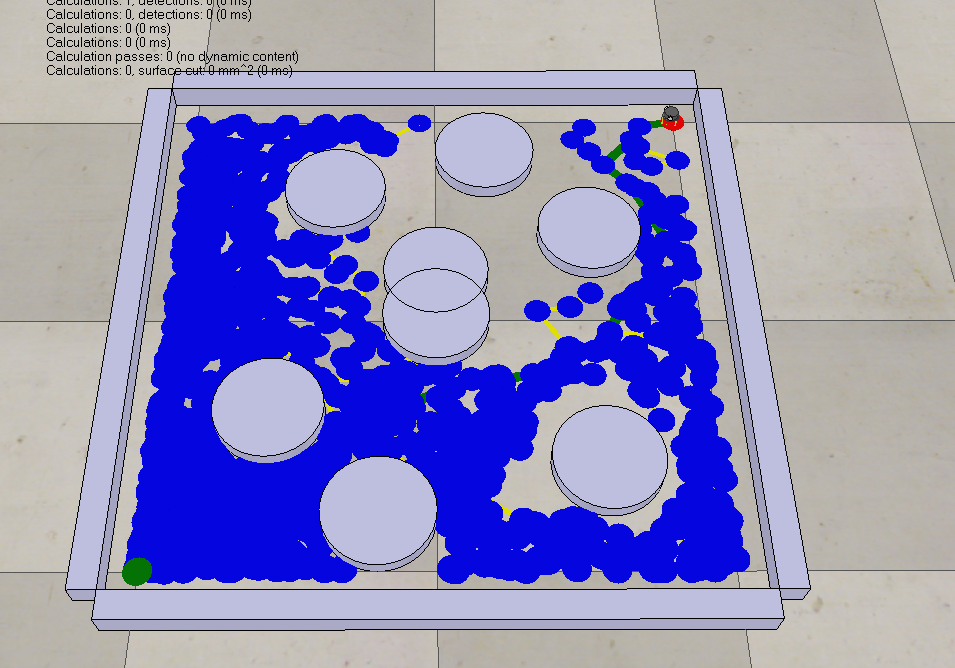
\includegraphics[width=0.7\linewidth, height=3.5cm]{screenshot.PNG}
\captionsetup{labelformat=empty}
\caption{V-Rep screen shot for RRT solution}
\end{subfigure}
\end{figure}
As shown in this figure, the program gives the path data as output which includes the nodes selected, edges to be travelled on, and cost to go. Final node will be goal node desired path data will have all the nodes in order as it goes further. Simulated in V-Rep with that data shows the motion of a kilo-bot reaching to the goal via path planned using MATLAB program. The optimal level of path planned depends on maximum number of iterations, size of the tree, provided and the factor $\epsilon$ value which specifies how far a neighbour node could possibly be and where to search specifically.
\subsubsection{3D implementation of RRT motion planner}
Updating the functions and the program by changing all the conditions from 2 dimensions to 3 dimensions, considering the Z axis and coordinates in space, 3D Algorithm is formed. Lot of obstacles were added on the map and even the nodes are considered to be in space with three coordinates. Range for finding neighbours is now spherical instead of circular,      

\begin{figure}[H]
\begin{subfigure}{0.5\textwidth}
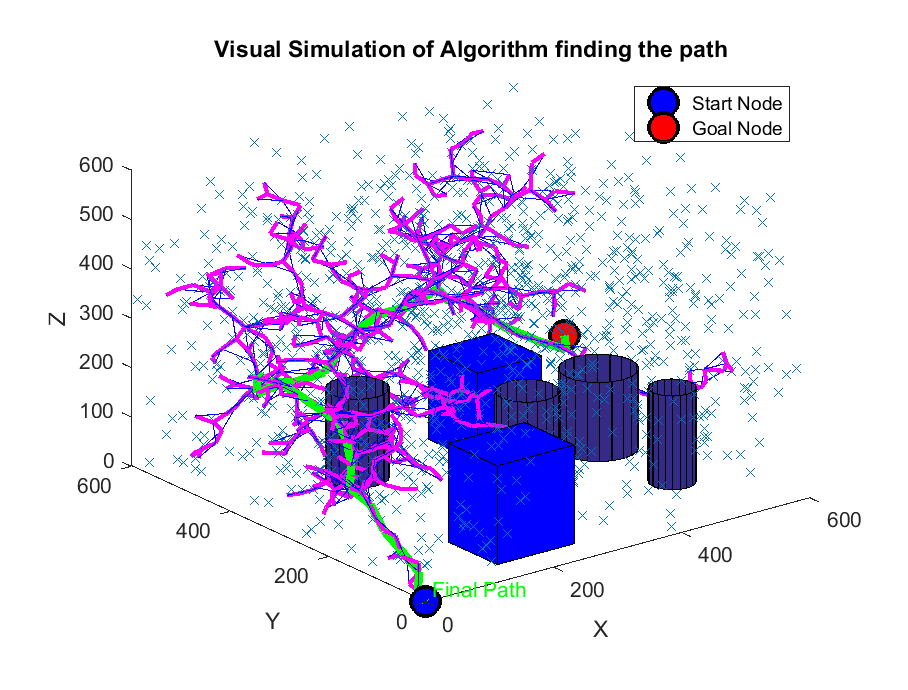
\includegraphics[width=0.8\linewidth, height=5cm]{RRT_LARGERTREE_RUN.eps}
\captionsetup{labelformat=empty}
\caption{RRT 3D in action}
\end{subfigure}
\begin{subfigure}{0.5\textwidth}
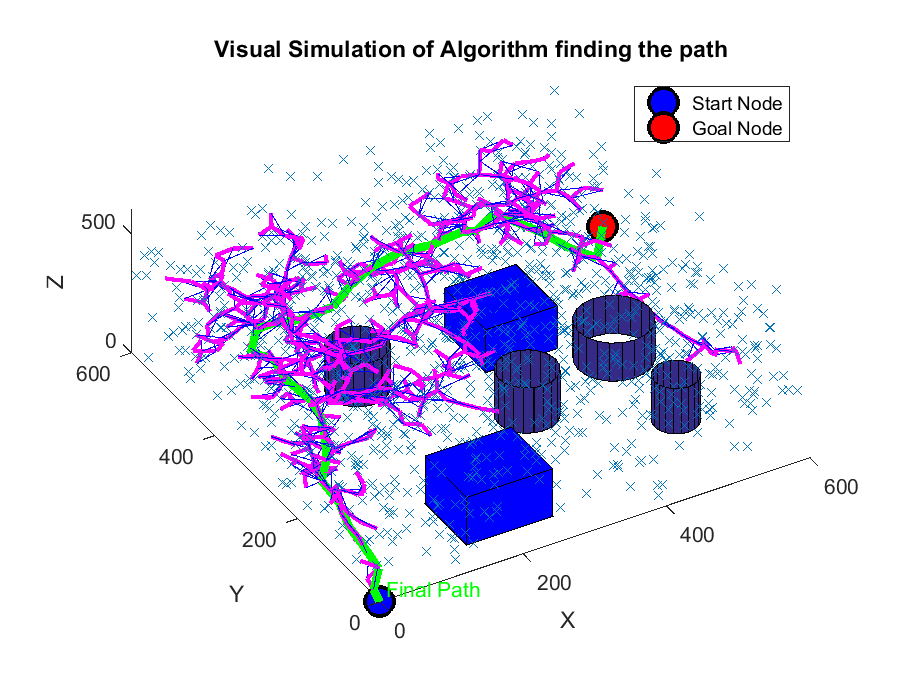
\includegraphics[width=0.8\linewidth, height=5cm]{RRT_LARGERTREE_RUN_VIEW.eps}
\captionsetup{labelformat=empty}
\caption{Different angle view}
\end{subfigure}
\end{figure}
The green colored line is the final path planned by the code, whereas the magenta colored line represents the tree and its branches. The blue cross symbols are all nodes generated randomly and sampled all over the map. Starting from the "Start node", exploring the random nodes and searching using a tree like structure, the algorithm finds for a good path to reach to the "Goal node" without any obstacle collision. 
\subsubsection{Changing parameters and variables}
For different start point and goal points, using higher number of nodes with larger size of  tree. Also, the criteria for searching in neighbourhood is reduced to explore more nodes within the limit. 
\begin{figure}[H]
\begin{subfigure}{0.5\textwidth}
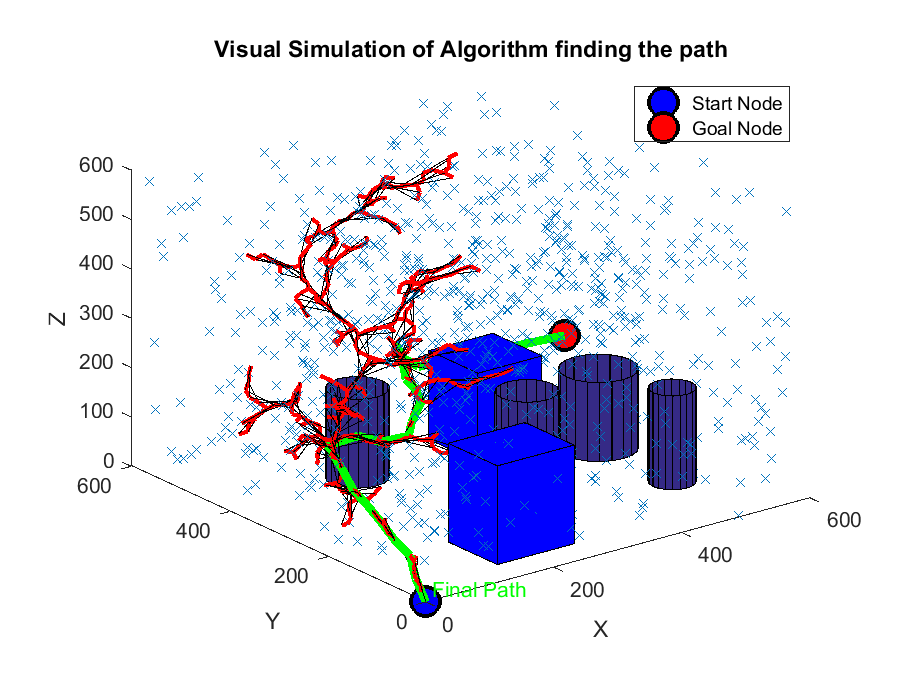
\includegraphics[width=0.8\linewidth, height=3.5cm]{RRT_RUN2.eps}
\captionsetup{labelformat=empty}
\caption{RRT 3D in action}
\end{subfigure}
\begin{subfigure}{0.5\textwidth}
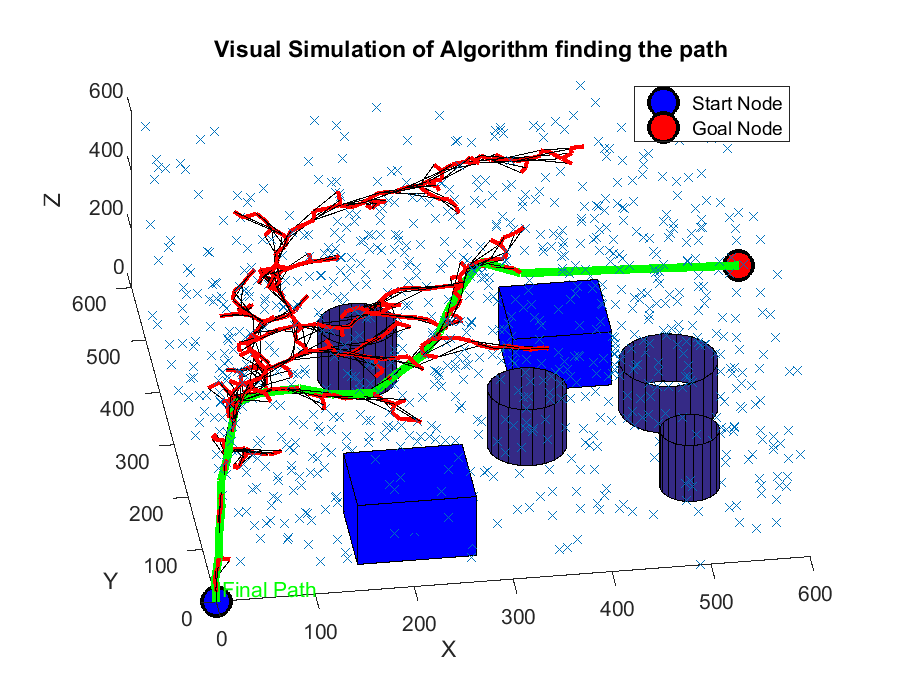
\includegraphics[width=0.8\linewidth, height=3.5cm]{RRT_RUN2_VIEW.eps}
\captionsetup{labelformat=empty}
\caption{Different angle view}
\end{subfigure}
\end{figure}
As it is clearly understandable from the simulation result that highly optimal solution with better accuracy is obtained. However, it took longer time to converge to this solution, so there is a need to compare the cost reduction and time taken to plan the path to have a perfect optimal solution. Having identified perfect values for each of the criteria and maximum size of the tree, $T$ and using those in MATLAB simulation, result is obtained using the same algorithm.

\begin{figure}[H]
    \centering
    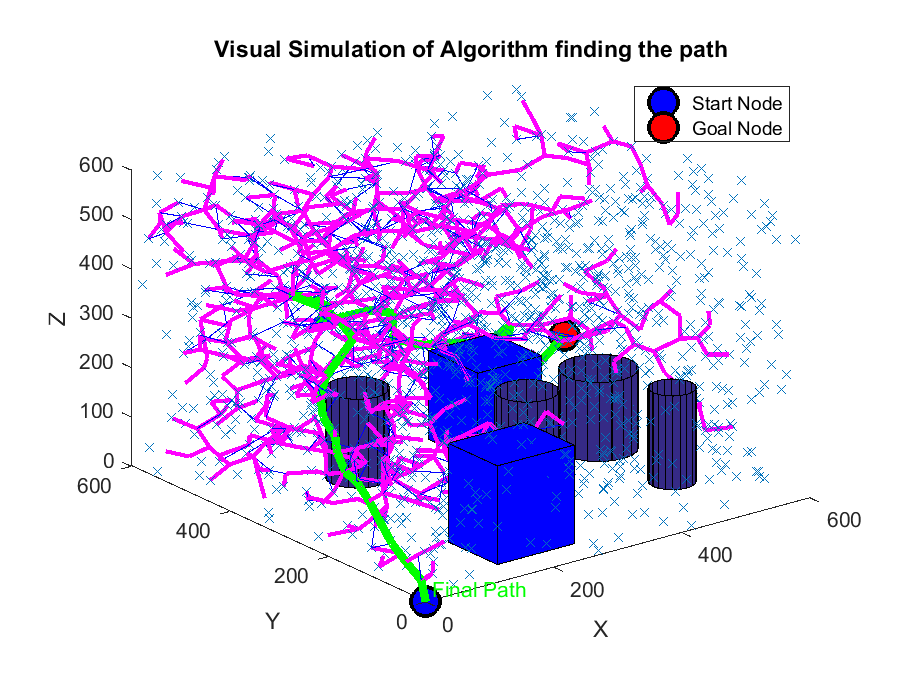
\includegraphics[scale=0.5]{RRT_RUN3.eps}
    \captionsetup{labelformat=empty}
    \caption{Implementing analyzed values in code}
\end{figure}

\subsubsection{3D RRT algorithm implemented on a ground vehicle }
For a mobile robot that can drive on ground only, same Algorithm is used except that all the Z-coordinates are assigned the value 'zero'. The program works in same manner as before just the change is that it creates branches on x-y plane and not in space. This algorithm could also be implemented on  an autonomous car to plan its path from one location to other. Next, Controls and Trajectory planning part of the mobile robot is considered and solved using Dynamics of model of a mobile robot.
\begin{figure}[H]
    \centering
    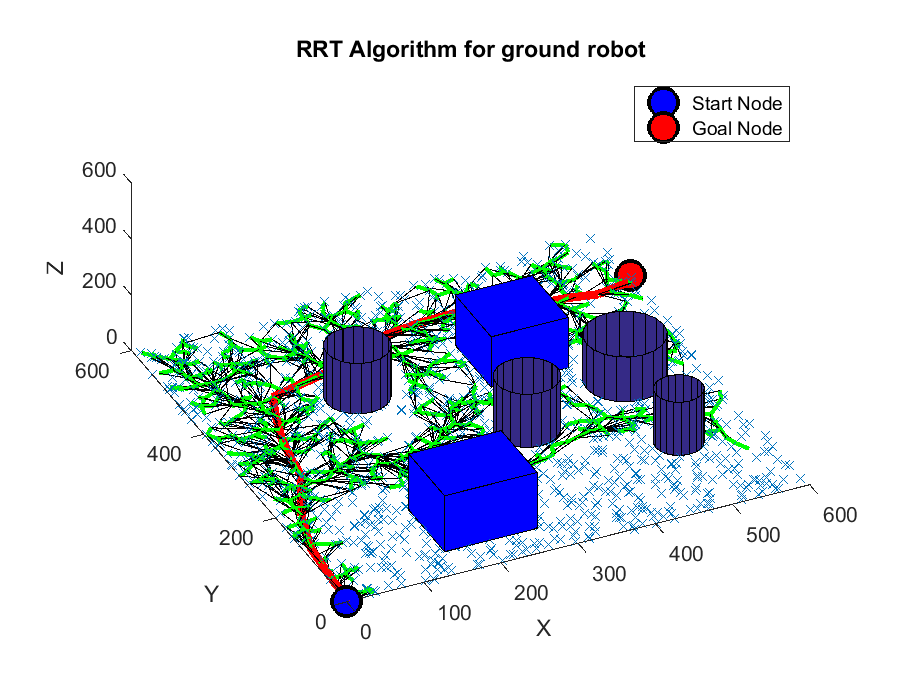
\includegraphics[scale=0.35]{RRT_GROUND_RUN.eps}
    \captionsetup{labelformat=empty}
    \caption{RRT motion planner for ground robot/vehicle}
\end{figure}

\subsection{Computational cost analysis for RRT algorithm}
Having studied, a paper about similar work done by PhD students at Department of Computer Science, COMSATS Institute of Information Technology, Lahore [10]. Experiments for  10 different runs were carried out in MATLAB code with changing number of iterations, varying the value of epsilon that restricts the movement within a certain distance, and varying the range in which algorithm searches for nearest neighbour nodes. For this experiment, simulation environment is developed using 64-bit MATLAB R2016b. The operating system used is 64-bit Windows 10. The test simulation runs for computational cost and performance evaluation are executed on a PC with Intel i5-7200 CPU @2.50GHz 2.70GHz and 8GB installed RAM.

\begin{center}
 \captionof{table}{Time taken for different number of maximum nodes allowed}
 \begin{tabular}{||c | c | c | c||} 
 \hline
Number of Iterations & \multicolumn{3}{|c|}{Time taken by MATLAB code to converge} \\
% Number of iterations  \\
 \hline
 \hline
 epsilon val & 10 & 20 & 50 \\  
 \hline
 200 & 5.6 & 4 & 8.9 \\ 
 \hline
 400 & 11.8 & 14 & 18 \\
 \hline
 600 & 20 & 29 & 29.5 \\
 \hline
 800 & 27 & 42 & 47 \\
 \hline
 1000 & 44 & 60 & 58 \\ 
  \hline
 1200 & 57 & 78 & 82 \\ 
 \hline
 1400 & 76 & 95 & 98.3 \\
 \hline
 1600 & 101 & 120 & 132 \\
 \hline
 1800 & 117 & 156 & 167 \\
 \hline
 2000 & 140 & 171 & 192.9 \\ 
 \hline
\end{tabular}
\end{center}

\begin{figure}[H]
    \centering
    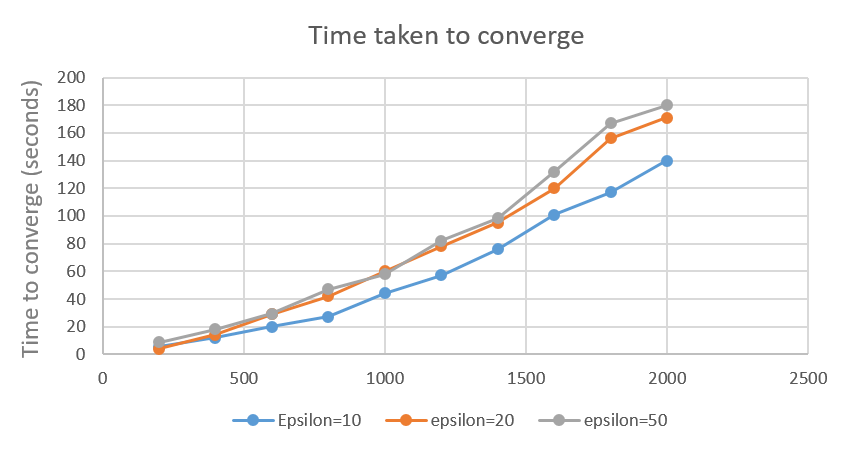
\includegraphics[scale=0.65]{Chart.png}
    \captionsetup{labelformat=empty}
    \caption{Graph for 'Time taken' vs 'Max allowed nodes'}
\end{figure}

It is clearly visible from the graph that as the value of epsilon increases, the time taken for code to run increases for equal number of iterations. However, completeness of search also increases along with epsilon value. But very high value is not recommended because of high time cost. So, optimal values for epsilon and the size of the tree, i.e. maximum number of allowed nodes in the map are needed to obtain a better solution. For epsilon value of 10, only 35\% of the map is covered by the search while for epsilon value of 50 almost 90\% of map area is covered. If epsilon value is taken as 25, search was executed by RRT planner within 80-84\% of the map area. So, 25 is a good value for having an optimal and probabilistic-ally complete solution.

The time taken by code to converge to solution is too high for larger size of tree. For 3000 iterations, code takes about 16-18 minutes to find a solution path. Based on this simulation experiments, when 2200-2500 number of nodes are allowed to plot, a solution is obtained faster compared to other values.There are better chances of getting a cost-optimal solution path if we use these values for the parameters in algorithm and perform the simulation and plan a path for the robot.

\newpage
\section{Study of dynamics and control for a robot model}
Firstly, non-holonomic constraints are added to robot to make the system more accurate and practical. The constraint that the vehicle will always move in the direction of axis of symmetry and not sideways which is obvious rule for any wheeled vehicle. Other two constraints comes from pure rolling motion of two wheels, no slip actions occur while motion of the wheels. These constraints are called non holonomic because of the reason that the equations of such constraints consists of velocity variables i.e. first differential terms along with position variables. This makes the equations non integrable and hence these are called non holonomic constraints. Also, these constraints are dealt differently then regular holonomic constraints, as these constraints reduces the number of equations of motion to one less than number of degrees of freedom. 
\\ I have used three non holonomic constraints in the system shown above to make the motion equations similar to a real actual mobile vehicle. These complexities were solved by using Euler-Lagrange approach to derive the equations of motion for this system.So, the Lagrangian is nothing but the sum of linear and rotational kinetic energies and was derived by solving for kinematics of the system and is as follows
\begin{equation}
\begin{split}
    L=T_1+T_2=\frac{1}{2}\biggl[m\dot{x}^2+m\dot{y}^2\biggr]+2*\biggl[\frac{1}{2}(m_w\dot{x}^2+m_w\dot{y}^2)\biggr]+\frac{1}{2}\sum(I)\dot{\phi}^2
\\
 +I_w(\dot{\theta_r}^2+\dot{\theta_l}^2)+m_gd_{og}\biggl[\dot{y_g}cos(\phi)-\dot{x_g}sin(\phi)\biggr]
\end{split}
\end{equation}
where I is the sum of moment of inertia of each of the components of robot.

Now, The dynamics of system are obtained using substitution of Lagrangian into Euler Lagrange equations, for the states defined by generalized coordinates.Thus, the dynamics of the system are represented by the following equations of motion

\[m\ddot{x_g}-m_gd_{og}(\ddot{\phi}sin(\phi)+{\dot{\phi}}^2cos(\phi))-\lambda_1sin(\phi)-\lambda_2cos(\phi)-\lambda_3cos(\phi)=0\]
\[m\ddot{y_g}-m_gd_{og}(\ddot{\phi}cos(\phi)+{\dot{\phi}}^2sin(\phi))+\lambda_1cos(\phi)-\lambda_2sin(\phi)-\lambda_3sin(\phi)=0\]
\[-m_gd_{og}(\ddot{x_g}sin(\phi)-\ddot{y_g}cos(\phi))+I\ddot{\phi}-d_{og}\lambda_1+b(\lambda_3-\lambda_2)=0)\]
\[I_w\ddot{\theta_r}+\lambda_2r=\tau_1\]
\[I_w\ddot{\theta_l}+\lambda_3r=\tau_2\]
\[M(q)\ddot{q}+V(q,\dot{q})=E(q)\tau-A^T(q)\lambda\]
which is obtained by separating each of the coefficients of inertia into M matrix, Constraint coefficients into A matrix, V is the other terms having position and velocity variables while E is just a transformation matrix. 
Thus, these matrices and vectors are obtained as follows, 
\begin{equation*}
M=
\begin{matrix}
m & 0 & -m_gd_{og}sin(\phi) & 0 & 0\\
0 & m & m_gd_{og}cos(\phi) & 0 & 0\\
-m_gd_{og}sin(\phi) & m_gd_{og}cos(\phi) & I & 0 & 0\\
0 & 0 & 0 & I_w & 0\\
0& 0& 0& 0 & I_w
\end{matrix}
\end{equation*}
\\
\begin{equation*}
V=
\begin{matrix}
-m_gd_{og}\dot{\phi}^2cos(\phi)\\
m_gd_{og}\dot{\phi}^2sin(\phi)\\
0\\
0\\
0
\end{matrix}
\end{equation*}

\begin{equation*}
E=
\begin{matrix}
 0&0\\0&0\\0&0\\1&0\\0&1
\end{matrix}
\end{equation*}
\begin{equation*}
A=
\begin{matrix}
-sin(\phi) & cos(\phi) & -d_{og} & 0 & 0\\
-cos(\phi) & -sin(\phi)& -b & r & 0\\
-cos(\phi) & -sin(\phi)& b & 0 & r\\
\end{matrix}
\end{equation*}
\\
while, $\tau$ and $\lambda$ are vectors representing the terms with torques and lambda's respectively having required dimensions and size.
\\
Now, solving this equation in MATLAB and simulating it, to get the graphs of the states with analysis. So, I gave different initial conditions for the mobile robot, and tried changing the parameters to obtain correct and good results. So, here I am showing different states plotted with different initial conditions mentioned. To plot the states, I used ODE45 backward integration, but using vectors for each of the states. It is not straightforward equations which could be used in ODE45. Mathematics required to solve this system is,

\[M(q)\ddot{q}+V(q,\dot{q})=E(q)\tau-A^T(q)\lambda\]
\[\ddot{q}=M^-1(E\tau-A^{T}\lambda-V)\]
This equation is not that simple to be solved by ODE45, I used an approach which includes forming a temporary vectors of the states and then equating the corresponding terms from vectors to the actual states and plotting them using those vector terms.
\\
\subsection{Dynamics Simulation results}
These are the states [x, y, $\phi$, $\theta_r$, $\theta_l$, $\dot{x}$, $\dot{y}$, $\dot{\phi}$, $\dot{\theta_r}$, $\dot{\theta_l}$] plotted,\\
1). Initial conditions are taken as all zeros

\begin{figure}[H]
\centering
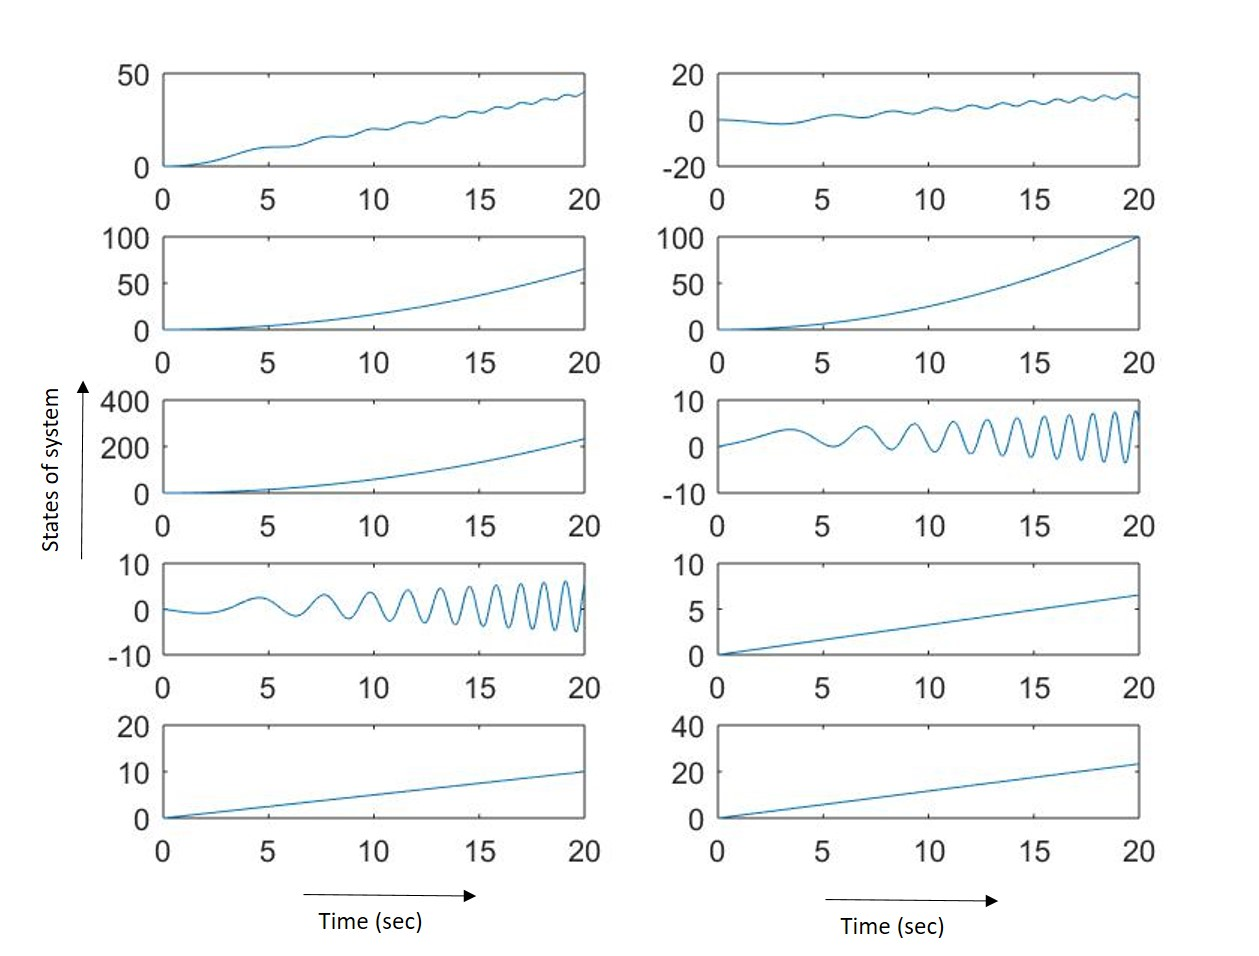
\includegraphics[width=0.6\textwidth]{zero.jpg}
\captionsetup{labelformat=empty}
\caption{States of system with all zero initial conditions}
\end{figure}

2). Initial condition for heading angle of vehicle is taken as $\phi=\pi/2$ while rest all are zeros,

\begin{figure}[H]
\centering
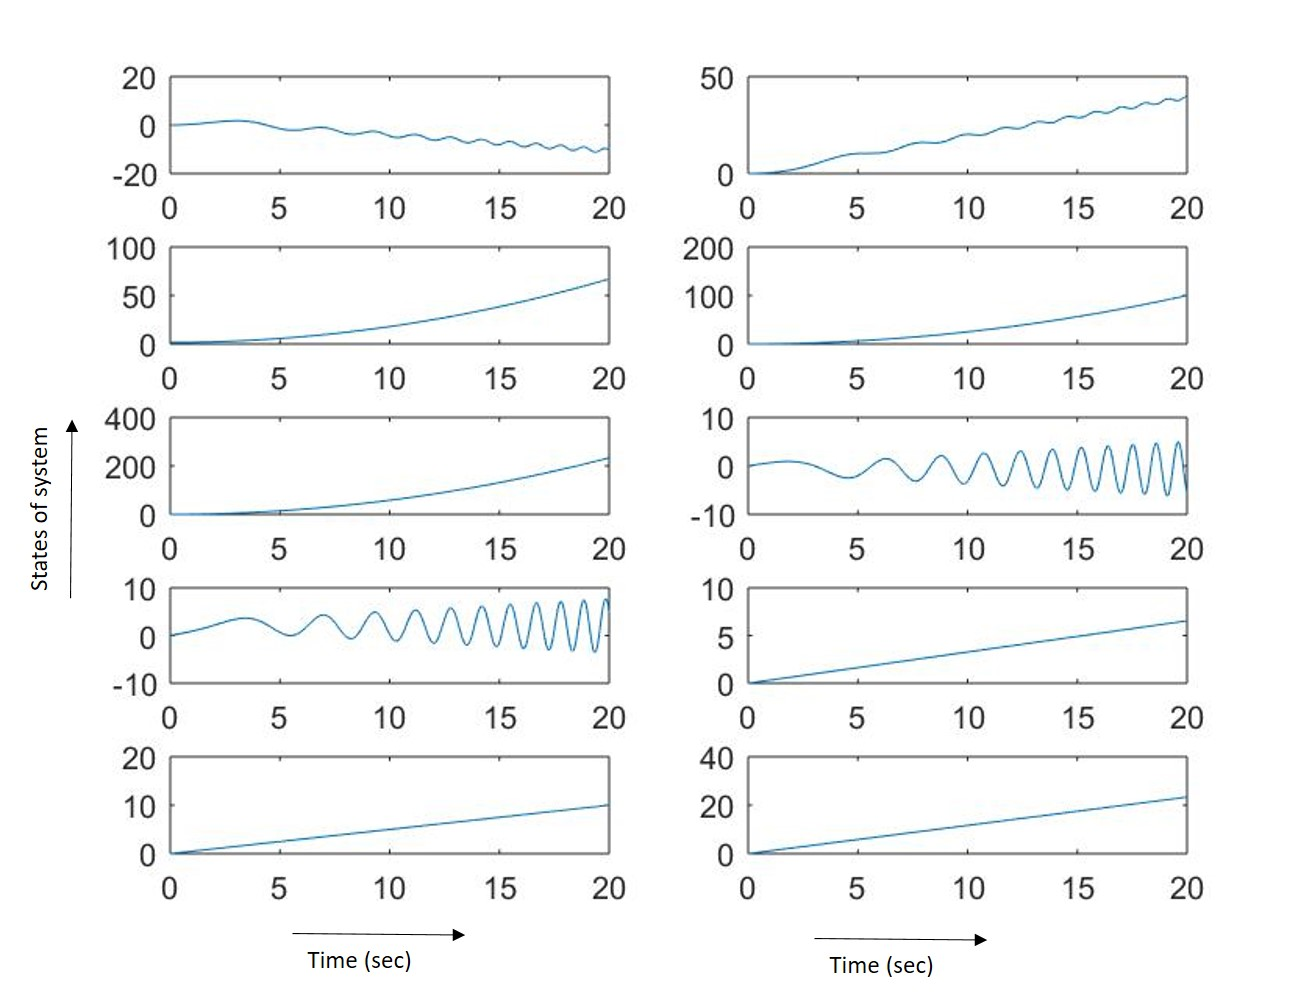
\includegraphics[width=0.6\textwidth]{piby2.jpg}
\captionsetup{labelformat=empty}
\caption{States with all initial conditions zero but heading angle 90 degrees initial conditions}
\end{figure}

3). Initial condition for heading angle of vehicle is taken as $\phi=\pi$ while rest all are zeros,
\begin{figure}[H]
\centering
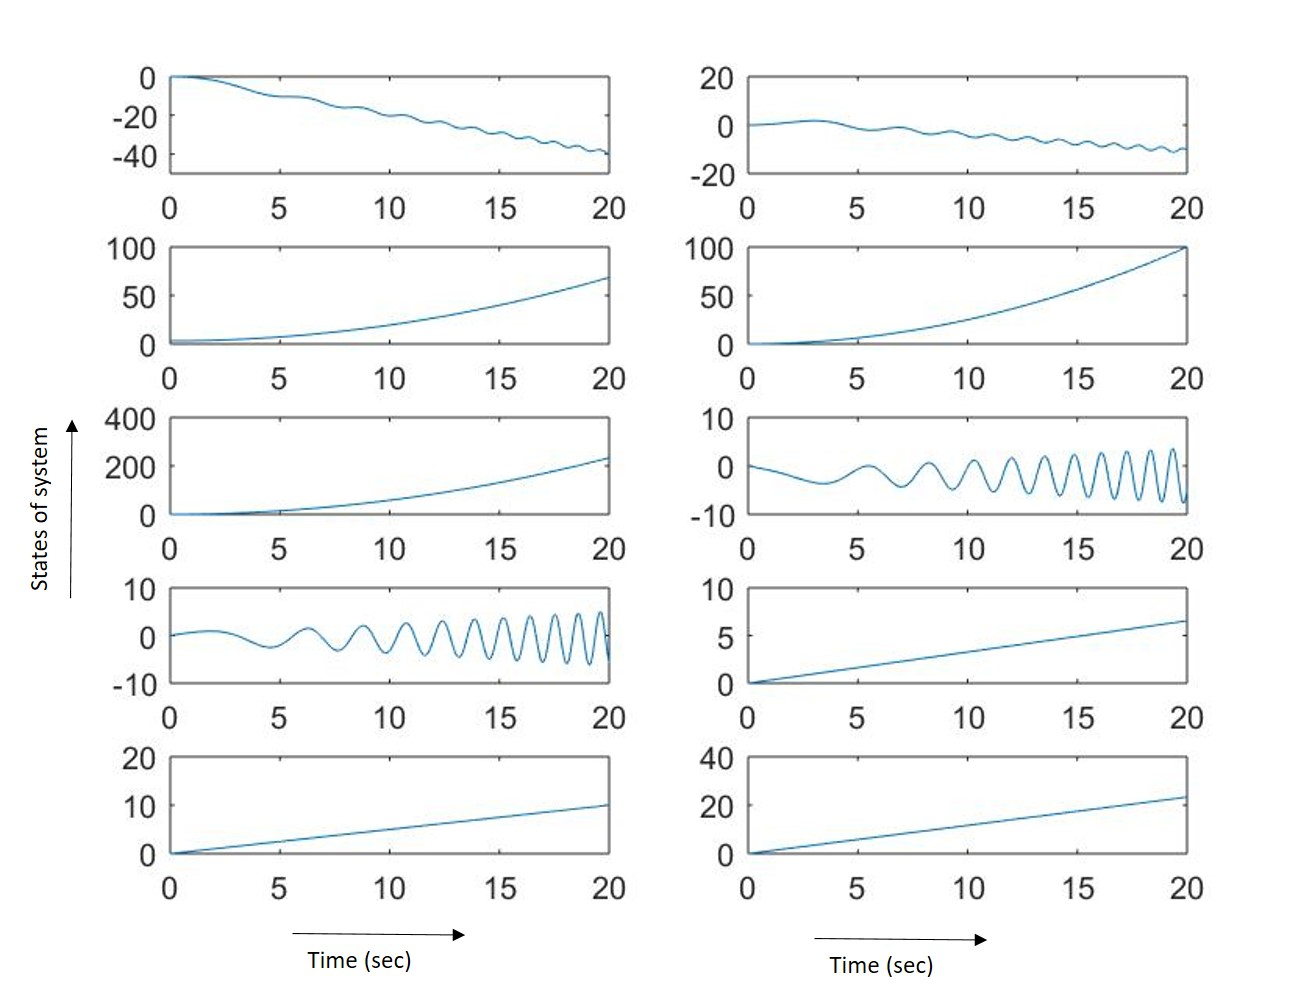
\includegraphics[width=0.6\textwidth]{pi.jpg}
\captionsetup{labelformat=empty}
\caption{States with all zero but heading angle 180 degrees initial conditions}
\end{figure}

4). Initial condition for heading angle of vehicle is taken as $\phi=3\pi/2$ while rest all are zeros,
\begin{figure}[H]
\centering
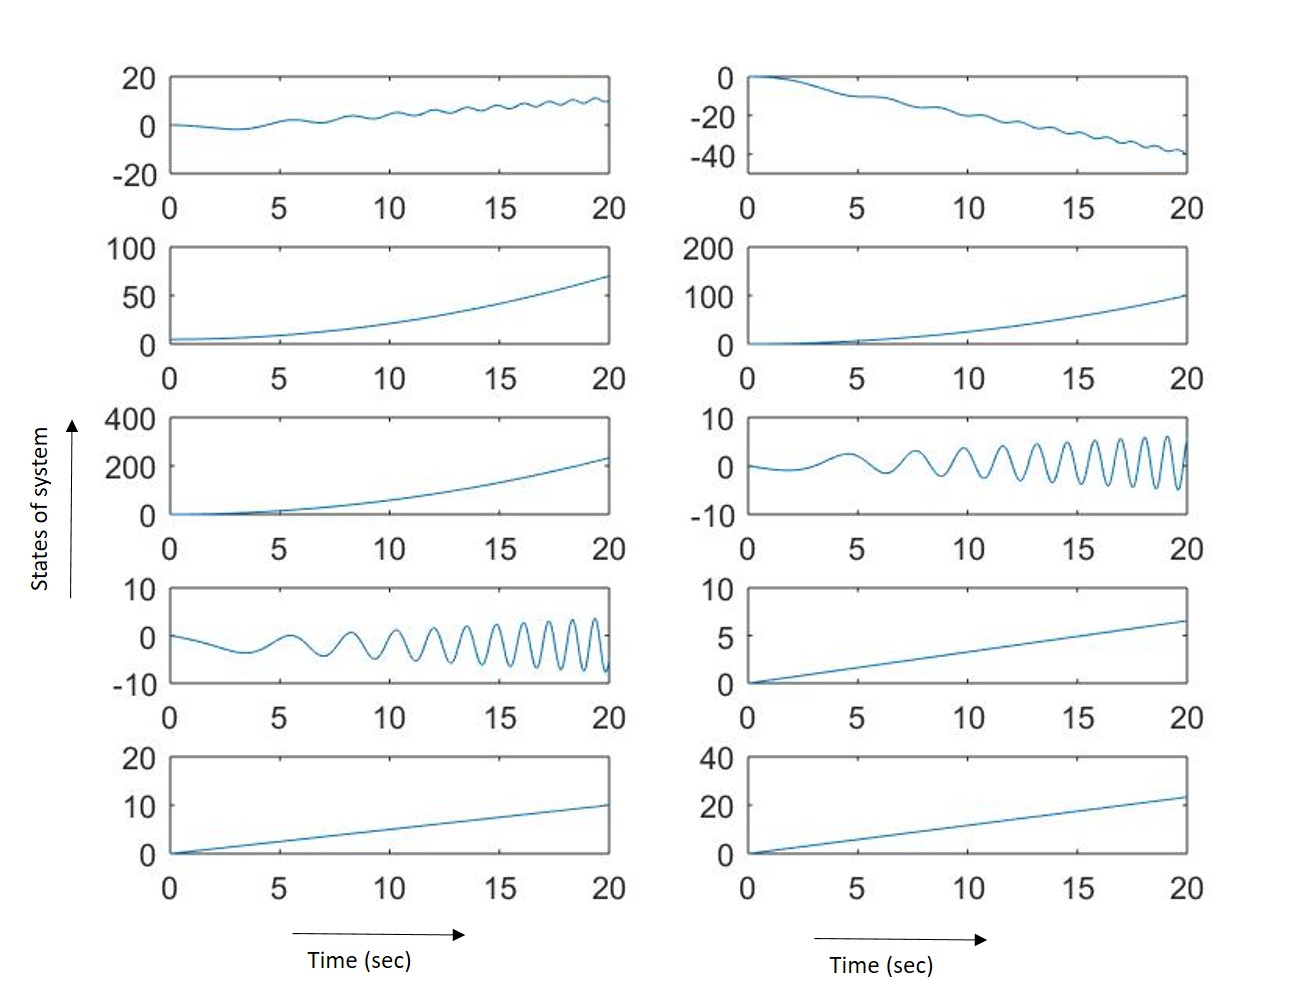
\includegraphics[width=0.6\textwidth]{3piby2.jpg}
\captionsetup{labelformat=empty}
\caption{States with all zero but heading angle 270 degrees initial conditions}
\end{figure}

\subsection{CONTROL}
First and easiest method comes in mind is Back stepping control technique, but it is not possible to solve the equations as those are not in the standard format which is required for a back stepping approach. So, Adaptive control method, which is also very popular while designing controller for mobile manipulators are selected and used to control the system.
\\
For course project of MAE 670 non linear control, Using the mathematics taught by Dr. T singh, I tried to obtain a control that stabilizes the system. But, it did not simplify itself into the linearized form and I had to use some other techniques which I learned from some references. So, first I solved the general dynamic equation which is showed earlier in the report by equating input torque matrix $\tau$ to all other terms on right side by inverting the equation. 
\[\tau=E(q)^-1(M(q)\ddot{q}+V(q,\dot{q})+A^T(q)\lambda)\]
However, this solution is not at all possible to design a controller. So, using a different approach, introducing a new vector S, which is formed by the knowledge of non holonomic constraint equations in matrix form. As, $A\dot{q}=0$, is the equation for the same, we know that vector $\dot{q}$ always lies in the null space of square matrix A. By using lie algebra technique, we can design some other linear combination of various other vectors which lies in null space of A matrix. And both of this equations will same and the new derived equation can be used in place of the original equation. So, I designed $AS(q)\nu(t)=0$, by saying $\dot{q}=S(q)\nu(t)$, where the vector $\nu$ is nothing but the 2 dimensional vector representing the angular velocities of both wheels.
Transforming the equations into new form by changing $\ddot{q}$ in terms of S and substituting it into the original dynamics equation. 
As, we need to do the pseudo inverse of the matrices which are not square matrix or which are non singular. So, to perform the pseudo inverse we multiply both sides by $S^T$ and obtain a new set of matrix equation.
\[S^T(M\dot{S}\nu+MS\dot{\nu}+V)=S^TE\tau\]
Performing some mathematical steps including pseudo inverse while inverting the equation and bringing all the terms at one side to equate, a new transformed state space equation could be obtained. The new transformed states are $x=[x, y, \phi, \theta_r, \theta_l, \dot{\theta_r}, \dot{\theta_l}]$
New transformed state space equation obtained is,
\begin{equation*}
\dot{x}=
(\begin{matrix}
S\nu\\(S^TMS)^-1(-S^TM\dot{S}\nu-S^T\nu)
\end{matrix})
+
(\begin{matrix}
0\\(S^TMS)^-1S^TE)
\end{matrix})\tau
\end{equation*}

Further, designing the torque vector for controlling, let us say \\
\begin{equation*}
\tau=[(S^TMS)^-1S^TE]^-1[u-(S^TMS)^-1(-S^TM\dot{S}\nu-S^TV)]
\end{equation*}
\\This is the control signal for torque, where just u is needed to be designed now based on non linearities in the equation.
Using this control signal for $\tau$, a new transformed state space equation is obtained as follows,
\[\dot{x}=f(x)+g(x)u\]
where f and g are two vectors consisting of $S\nu$ and I parts with other terms as zero.\\
So, as n-m states in the state space equation are zeros, full information cannot be obtained for feedback. So input-output linearization is required to solve for the control, which brings in view the necessity of  output equation. Thus, providing a reference desired output equation, we can solve the system using zero dynamics and design an adaptation law based on the results. 
I followed the zero dynamics method given in a book called “Adaptive Control Tutorial” by  Petros Ionnou and Baris Fidan. Obtained the Jacobian of matrix and solved for output equation which gave the adaptation law as $u=\Phi^-1(v_{ref}-\dot{\Phi}\nu)$
where, $\Phi$ represents the matrix formed using the Jacobian of system of zero dynamics.\\
Using reference position $(x_{error}, y_{error})$ as my output equation, where the error position comes from the difference between the actual and desired or reference position components. 

Overall approach block diagram, I created using Simulink tool of MATLAB for this control algorithm can be shown as below, 
\begin{figure}[H]
\centering
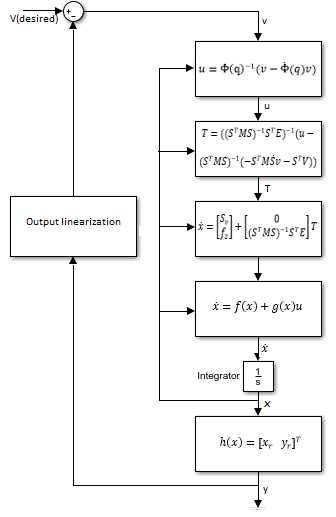
\includegraphics[width=0.4\textwidth]{final__1_.PNG}
\captionsetup{labelformat=empty}
\caption{Block Diagram of control algorithm using Simulink}
\end{figure}

\subsubsection{Simulation of Controller}
After implementing the controller in system model, simulating the system in MATLAB to see how is the performance of the controller is affecting the system model.

\begin{figure}[H]
\begin{subfigure}{0.5\textwidth}
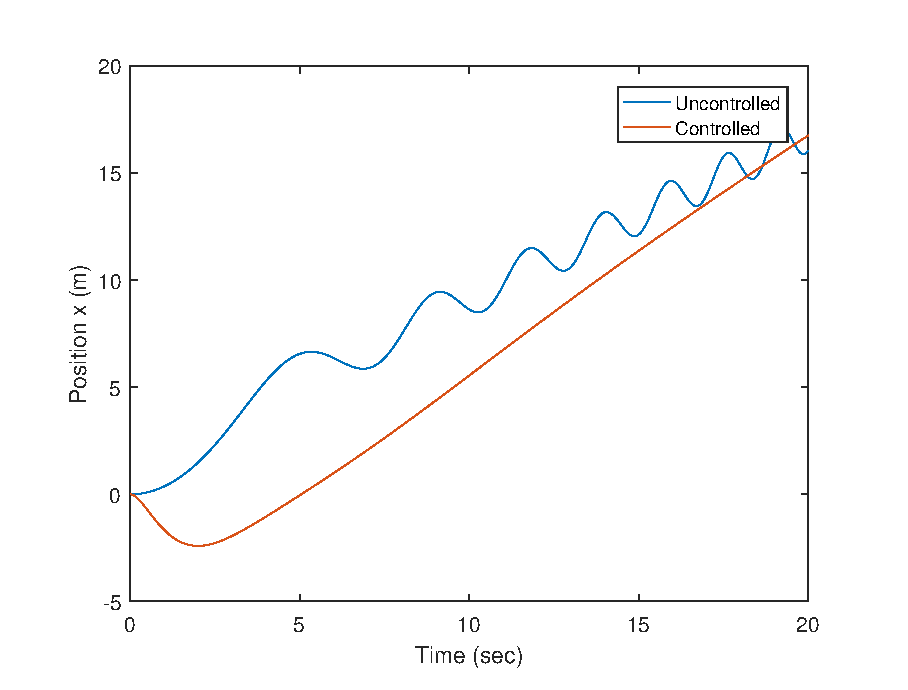
\includegraphics[width=0.7\linewidth, height=3.5cm]{state_x.eps}
\captionsetup{labelformat=empty}
\caption{The x position of robot}
\end{subfigure}
\begin{subfigure}{0.5\textwidth}
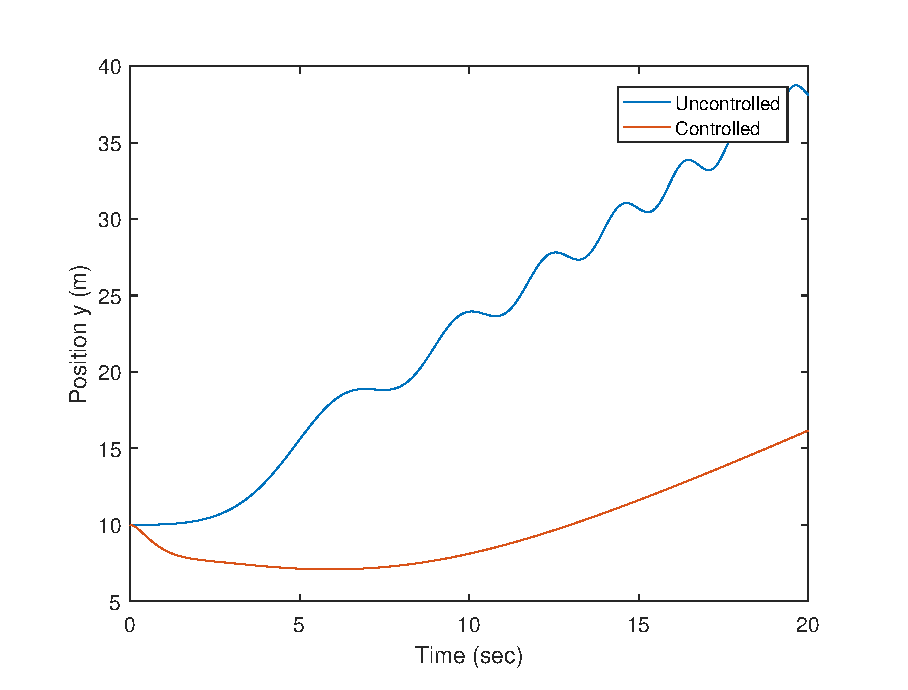
\includegraphics[width=0.7\linewidth, height=3.5cm]{state_y.eps}
\captionsetup{labelformat=empty}
\caption{The y position of robot}
\end{subfigure}
\end{figure}

As, predictable all the oscillations of the position states of system are eliminated by controller and also, the robot goes in the controlled direction as per the reference trajectory defined.
Now, the angle of the vehicle, 
\begin{figure}[H]
\centering
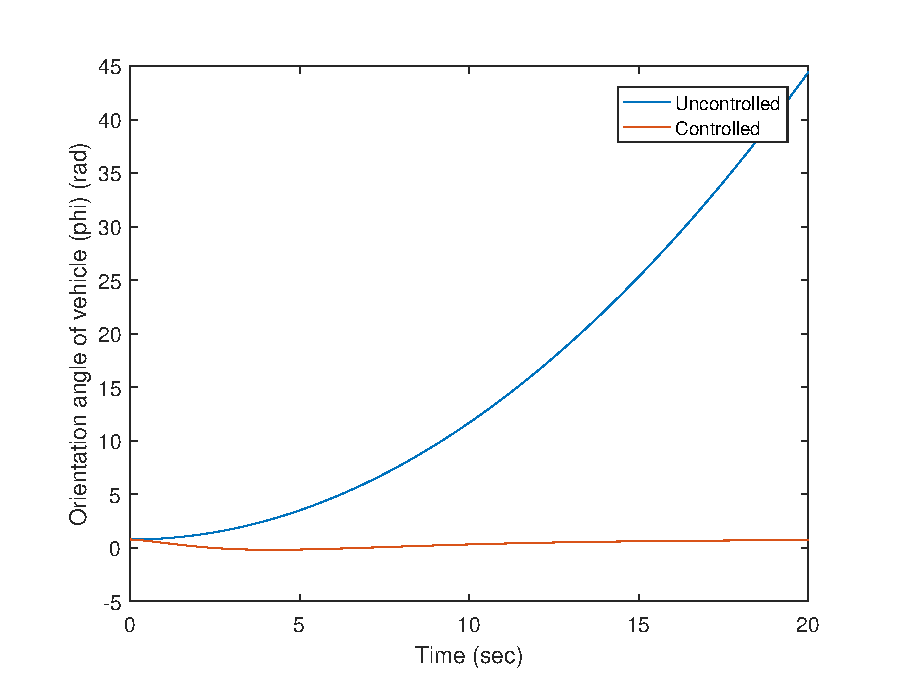
\includegraphics[width=0.3\textwidth]{state_phi.eps}
\captionsetup{labelformat=empty}
\caption{Controlled state of heading angle of vehicle}
\end{figure}

\begin{figure}[H]
\begin{subfigure}{0.5\textwidth}
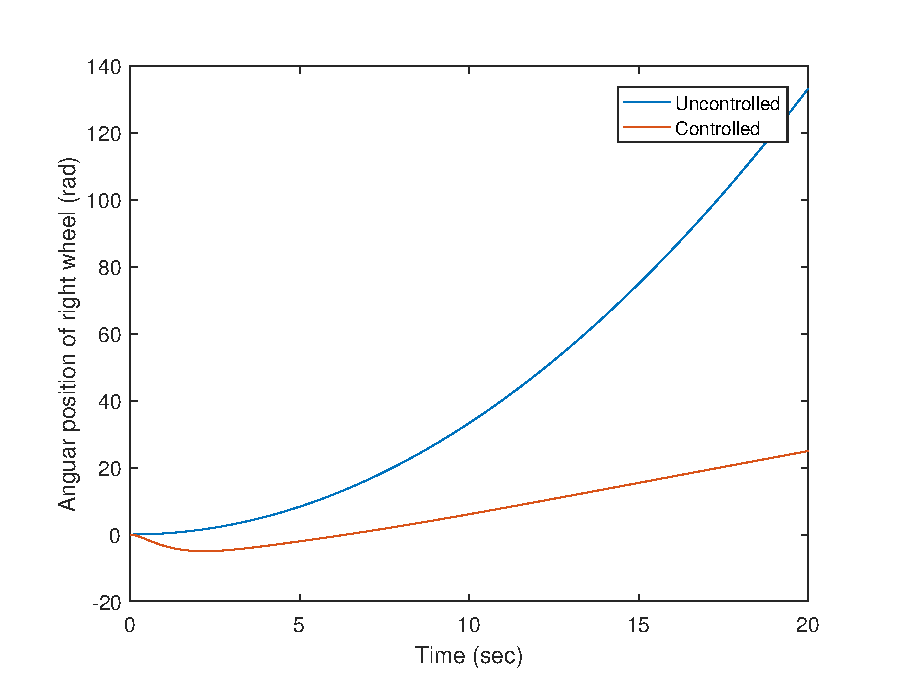
\includegraphics[width=0.7\linewidth, height=3.5cm]{state_theta_r.eps}
\captionsetup{labelformat=empty}
\caption{Angular positions of right wheel of the vehicle plotted}
\end{subfigure}
\begin{subfigure}{0.5\textwidth}
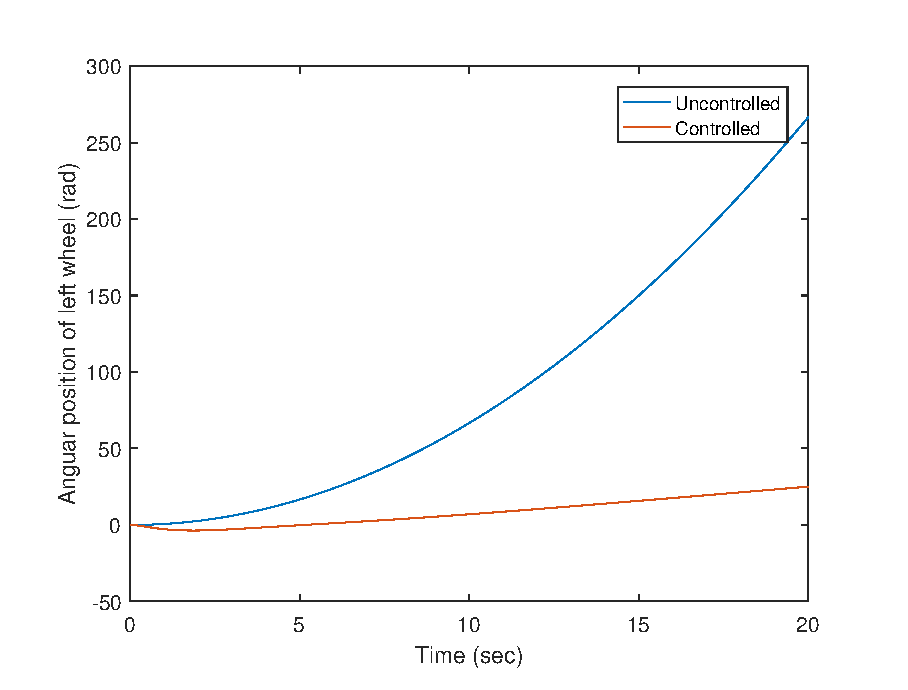
\includegraphics[width=0.7\linewidth, height=3.5cm]{state_theta_l.eps}
\captionsetup{labelformat=empty}
\caption{Angular positions of left wheel of the vehicle plotted}
\end{subfigure}
\end{figure}

So, the angles are controlled and forced to move slowly so that robot can follow the desired path given as input by reducing the errors. The heading angle is quite stable after implementation of controller in the system. Moving further, showing the simulations of input signals which are the angular velocities of both wheels controlled by torque signal given from the controller.

\begin{figure}[H]
\begin{subfigure}{0.5\textwidth}
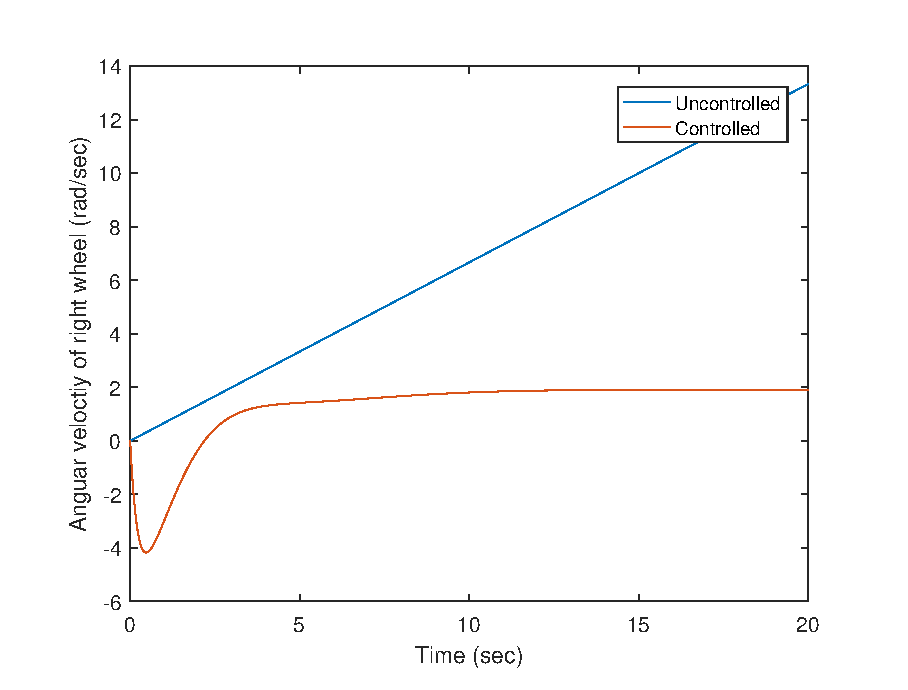
\includegraphics[width=0.7\linewidth, height=3.5cm]{control_on_right_wheel.eps}
\captionsetup{labelformat=empty}
\caption{Input/Control signal for the right wheel of vehicle}
\end{subfigure}
\begin{subfigure}{0.5\textwidth}
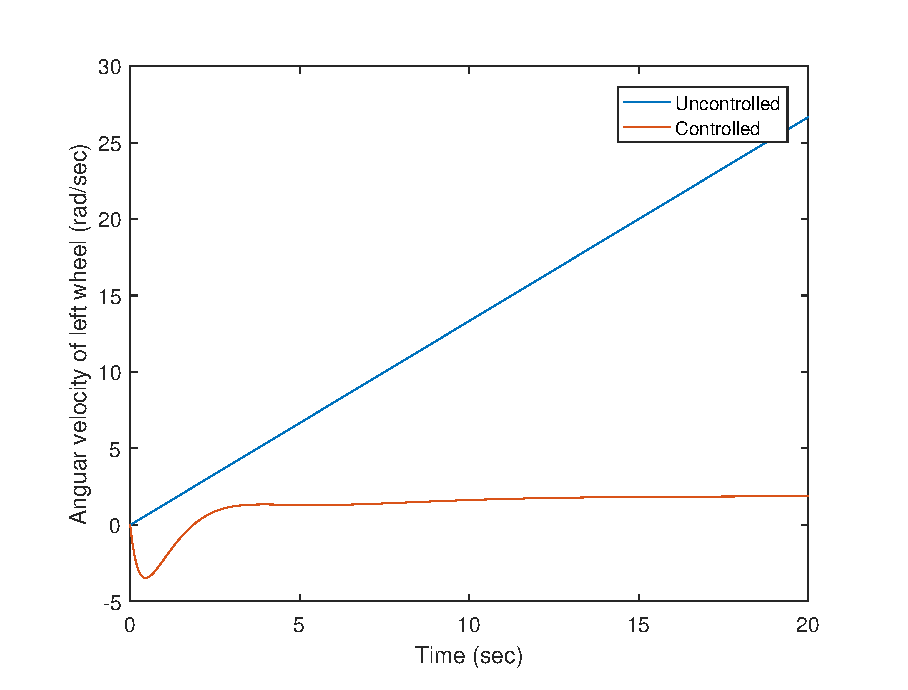
\includegraphics[width=0.7\linewidth, height=3.5cm]{control_on_left_wheel.eps}
\captionsetup{labelformat=empty}
\caption{Input/Control signal for the left wheel of vehicle}
\end{subfigure}
\end{figure}
Finally, the angular rates of wheels are controlled and the signal goes to stable state within a very short duration of time.
\begin{figure}[H]
\begin{subfigure}{0.5\textwidth}
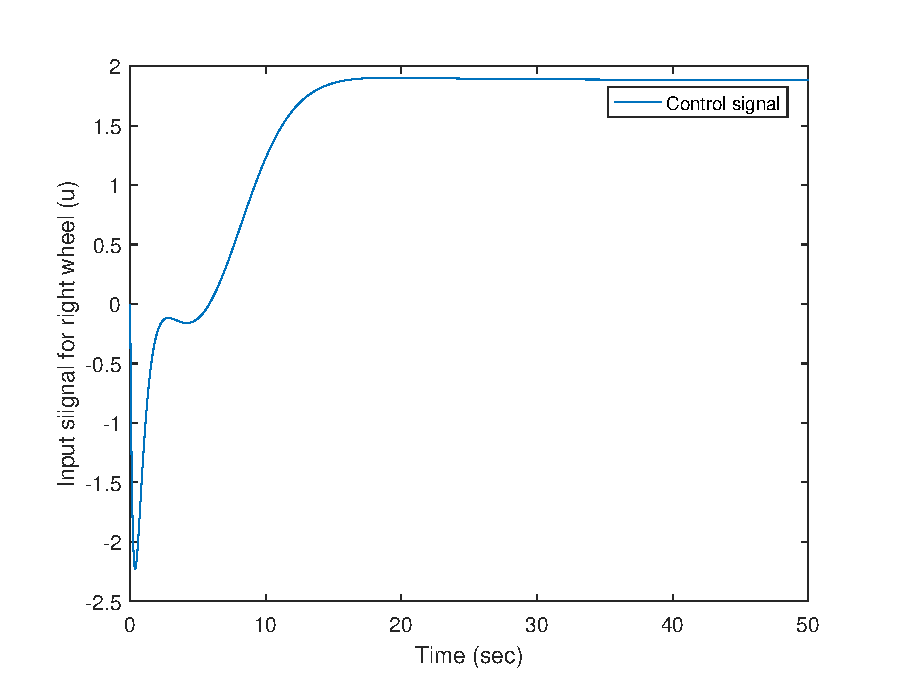
\includegraphics[width=0.7\linewidth, height=3.5cm]{state_theta_r_dot.eps}
\captionsetup{labelformat=empty}
\caption{Graph- angular speed of right wheel}
\end{subfigure}
\begin{subfigure}{0.5\textwidth}
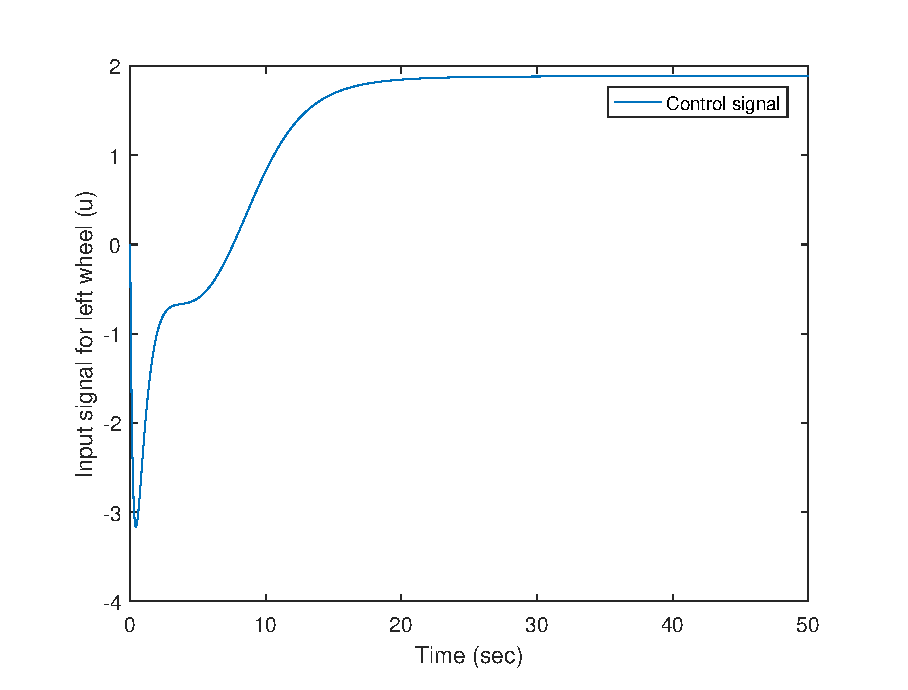
\includegraphics[width=0.7\linewidth, height=3.5cm]{state_theta_l_dot.eps}
\captionsetup{labelformat=empty}
\caption{Graph- angular speed of left wheel}
\end{subfigure}
\end{figure}
\newpage

\section{Pick and place application}
\subsection{Robot model - 'Youbot'}
The robot selected for this project is Youbot model from 'Kuka robotics' company. The model has 4 mecanum wheels on the base and a 5-joint manipulator mounted on it. The mecanum wheels make the robot capable of omnidirectional movement, so that the robot can move in any direction without any constraints. Also, manipulator has five number of joints which makes it more flexible and easy to perform the desired tasks.

\begin{figure}[H]
\centering
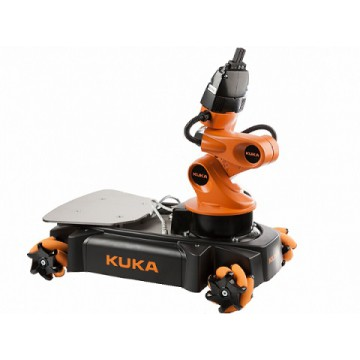
\includegraphics[width=0.5\textwidth]{kuka-youbot-robot-mobile-omni-directionel-avec-bras.jpg}
\captionsetup{labelformat=empty}
\caption{Robot model used for pick and place problem.\\ (\footnotesize Image credits: Generation Robots, https://www.generationrobots.com/en/402093-kuka-youbot-robot-mobile-omni-directionel-avec-bras.html)}
\end{figure}

\subsection{Kinematics}
Having studied kinematics of this model, the states of the robot model is considered as following, 
\begin{equation}
    q=[\phi, x, y, J_1, J_2, J_3, J_4, J_5, \theta_1, \theta_2, \theta_3, \theta_4, p]
\end{equation}
where $\phi$ s the heading angle of vehicle, and $x$ and $y$ represents the location of base vehicle,
	             $J_i$'s represents the joint position of  the manipulator, and 
	           $\theta_i$'s represents position of 4 wheels 
The thirteenth state, $p$ is considered when generating the reference trajectory, which is the state of gripper. It can only have two values, ‘0’ for open or ‘1’ for  closed.

Inputs required by the system includes
\begin{enumerate}
    \item Initial and final configuration of end effector
\item Initial and final position of cube
\item Number of reference configurations per time step
\end{enumerate}

After number of iterations, results are  obtained in form of output and is as follows,
\begin{enumerate}
    \item It gives reference trajectory in form of 13 states in a row. 
\item It gives error calculated by comparing desired next state and obtained trajectory state 
\item Number of rows of the csv file depends on the number of configurations considered per time step.
\end{enumerate}

Lie algebra principles and screw theory based calculations are performed in the program. Implementing the PI feedback controller, error was reduced to zero and system stabilizes within a certain interval without any overshoot. Performing different simulations, values of PI controller gain values are confirmed to be 
\begin{equation}
    K_P = 1.5,  K_I = 1.5 
\end{equation}   

\begin{figure}[H]
\centering
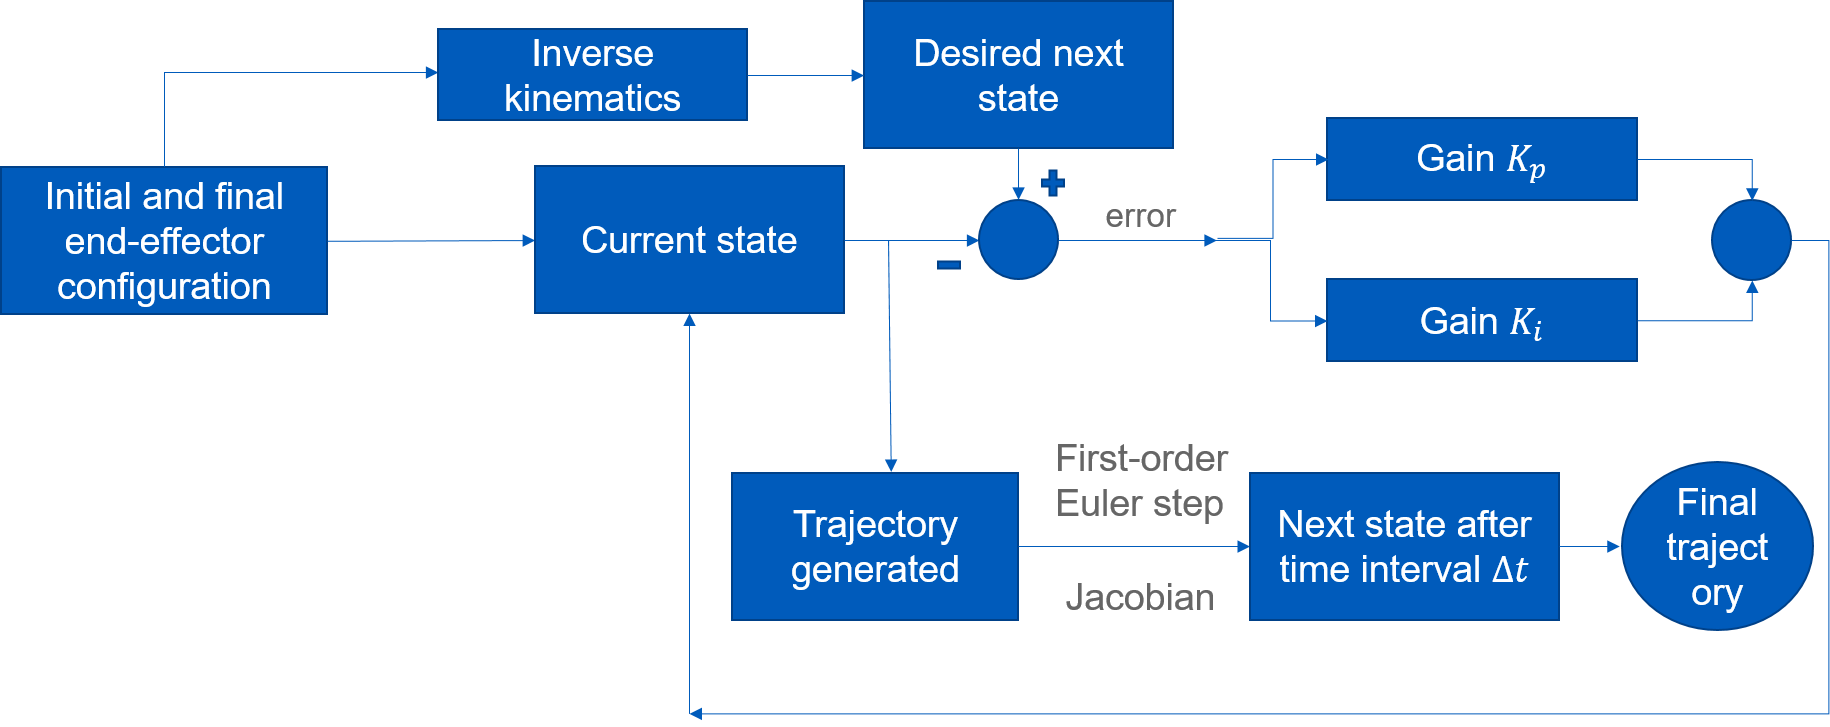
\includegraphics[width=0.9\textwidth]{Picture2.png}
\captionsetup{labelformat=empty}
\caption{Block diagram of the system}
\end{figure}

Other  initial conditions considered for simulation purpose are as following,
The initial configuration of the cube to be picked is taken as
\begin{equation}
    (x_i, y_i, \theta_i) = (1 m, 1 m, 0 rad)
\end{equation}
   while final/desired configuration of the cube is 
\begin{equation}
    (x_f, y_f, \theta_f) = (0 m, -1 m, -\pi/2 rad)
\end{equation}
 
 The simulated time for V-Rep video to calculate between each line of the csv file is 0.01 second (10 milliseconds)

 
\begin{figure}[H]
\centering
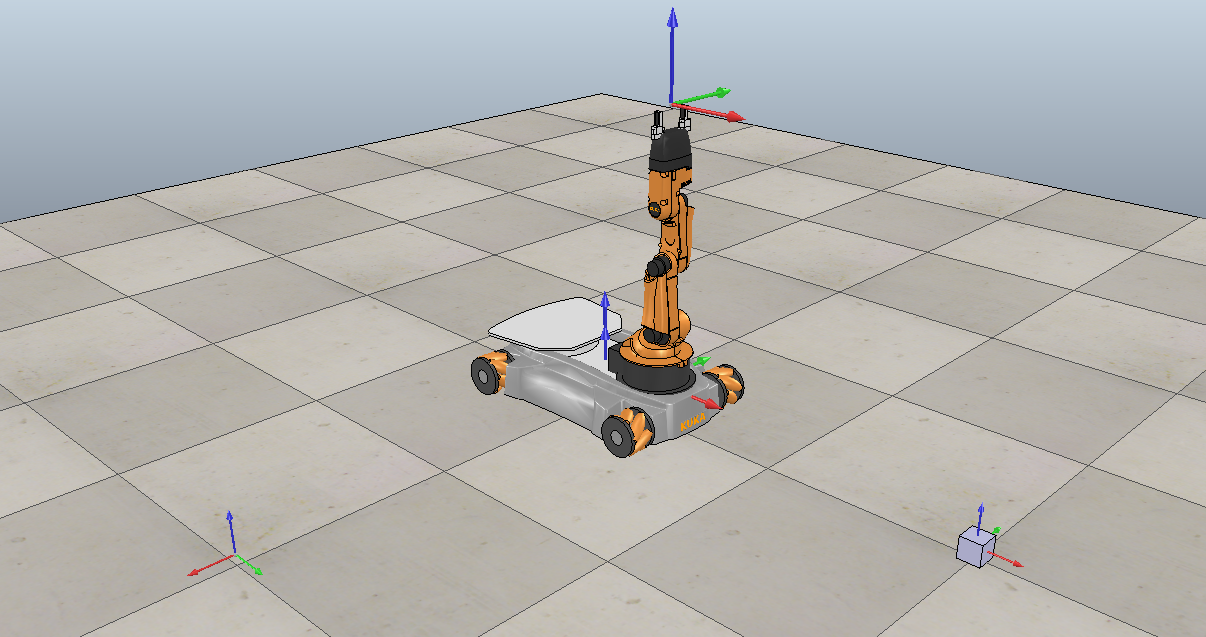
\includegraphics[width=0.5\textwidth]{Initial_vrep_simulation.PNG}
\captionsetup{labelformat=empty}
\caption{Simulation screen shot at initial conditions}
\end{figure}
 
\begin{figure}[H]
\centering
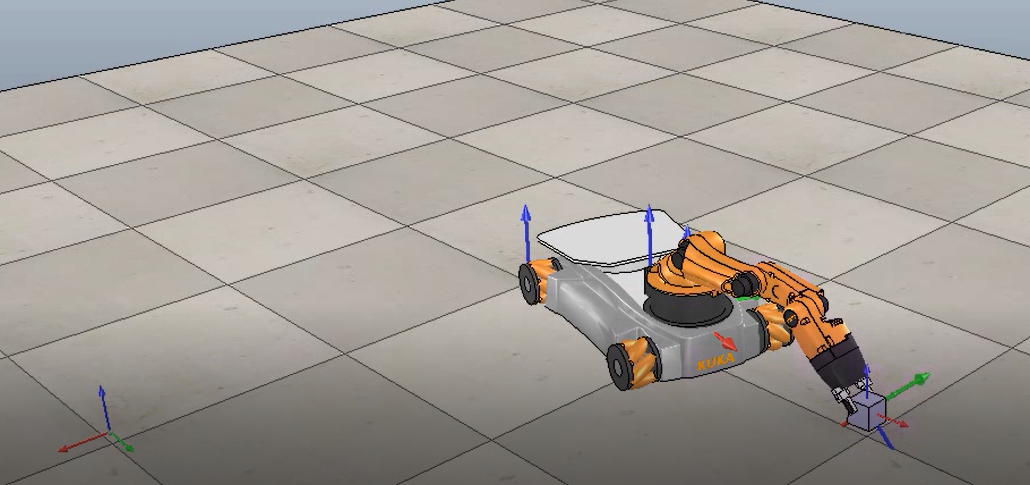
\includegraphics[width=0.5\textwidth]{first_end.PNG}
\captionsetup{labelformat=empty}
\caption{screen shot while youbot picks the object up}
\end{figure}
 
\begin{figure}[H]
\centering
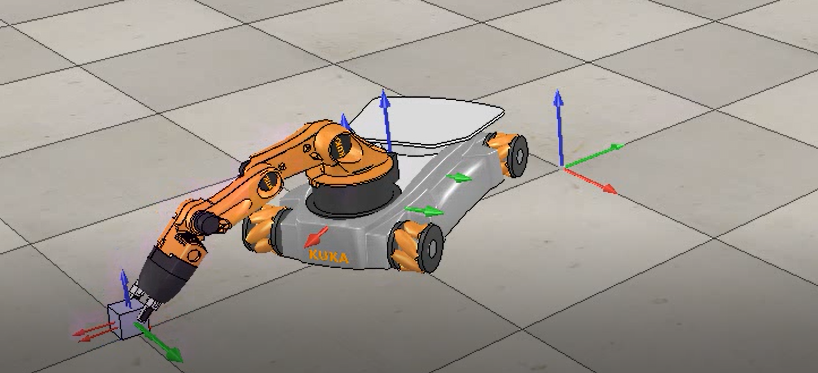
\includegraphics[width=0.5\textwidth]{final_end.PNG}
\captionsetup{labelformat=empty}
\caption{screen shot of 'youbot' placing object at desired position}
\end{figure}


\newpage
\section{Conclusion}
Hence, Motion Planning Algorithms were studied, analyzed and implemented on simulated mobile robot model. Planners including A*, PRM, RRT, RRT* were formulated based on different requirements of the robot. Various parameters used in each of these algorithms were analyzed and proper values obtained and simulated to see how modifications improved the results of motion planning. Dynamic modelling and controlling the system is another aspect which helps in better understanding the system model. After combining planning and controlling part, a mobile robot can work and perform the jobs desired. Any type of robots, whether it is an industrial manipulator robot, or a mobile vehicle like robot, an autonomous cars or hybrid models like EOD robots are made operable using these techniques modified and/or developed in this Project. These Methods and Techniques will be very useful for future progress and development in the field of Robotics.  
\newpage

\begin{thebibliography}{9}
\bibitem{Modern Robotics.} 
Lynch, K.M., Park, F.C.
\textit{Modern Robotics.}. 
Cambridge University Press, Cambridge (2017)
\bibitem{LaValle, S. M.} 
LaValle, S. M.
\textit{‘Rapidly-Exploring Random Trees: A New Tool for Path Planning’}
TR 98-11, Computer Science Department, Iowa State University, Oct. 1998.
\bibitem{Karaman, Sertac, and Emilio Frazzoli.} 
Karaman, Sertac, and Emilio Frazzoli.
\textit{"Incremental sampling-based algorithms for optimal motion planning."}
Robotics Science and Systems VI 104 (2010).
\bibitem{Steven M. LaValle} 
Steven M. LaValle
\textit{"Planning Algorithms"}
University of Illinois, Cambridge University
\bibitem{Siegwart, Roland,and Illah Nourbakhsh.} 
Siegwart, Roland, and Illah Nourbakhsh.
\textit{"Introduction to autonomous mobile robots"}
Library of Congress Cataloging-in-Publication Data
\bibitem{Sanjay K Sharma, Robert Sutton, Amit Motwani and Andy Annamalai} 
Sanjay K Sharma, Robert Sutton, Amit Motwani and Andy Annamalai
\textit{"Non-linear control algorithms for an
unmanned surface vehicle"}
J Engineering for the Maritime Environment
2014, Vol. 228(2) 146–155
\bibitem{W.E. Dixon, M.S. de Queiroz, F. Zhang and D.M. Dawson} W.E. Dixon, M.S. de Queiroz, F. Zhang and D.M. Dawson
\textit{"Tracking Control of Robot Manipulators with Bounded Torque Inputs*"}
Department of Electrical and Computer Engineering, Clemson University, Clemson, SC 29634-0915 (USA)
\bibitem{Yoshio Yamamoto and Xiaoping Yun} 
Yoshio Yamamoto and Xiaoping Yun
\textit{Coordinating
locomotion and manipulation of a mobile manipulator}. 
General robotics and active sensory perception (GRASP) laboratory IEEE 1992
\bibitem{Jean-Jacques E, Slotine Weiping Li} 
Jean-Jacques E, Slotine Weiping Li
\textit{Applied Nonlinear Control}
\bibitem{Iram Noreen, Amna Khan, Zulfiqar Habib} 
Iram Noreen, Amna Khan, Zulfiqar Habib
\textit{A Comparison of RRT, RRT* and RRT*-Smart Path Planning
Algorithms, IJCSNS International Journal of Computer Science and Network Security, VOL.16 No.10, October 2016}
\bibitem{Northwestern University} 
Northwestern University
\url{"http://hades.mech.northwestern.edu/index.php/Coursera_Resources"}
\bibitem{Latex Instructions} 
Overleaf Latex Instructions
\url{"https://www.overleaf.com/learn/"}
\bibitem{Wikipedia} 
Wikipedia
\url{"https://www.wikipedia.org/"}
\bibitem{StackX} 
Latex Stack Exchange
\url{"https://tex.stackexchange.com/"}
\end{thebibliography}

\end{document}